\documentclass[20pt,landscape,footrule,headrule]{foils}
\usepackage[usenames]{color}
\usepackage[export]{adjustbox}
\usepackage{latexsym}
\usepackage{amsmath}
\usepackage{graphicx,color}  %needed to \includegraphics
\usepackage{amssymb}
\usepackage{multirow}
\usepackage{multicol}
\usepackage{polynom}
\usepackage{tabularx}
\usepackage{threeparttable}
\usepackage{siunitx}
\usepackage{ulem}
\usepackage{colortbl}
\usepackage{multirow}
\usepackage{hhline}
\usepackage{calc}
\usepackage{array}
%\usepackage{caption}
\newcommand{\newl}{\newline\newline}
\newcommand{\GN}{\mathbb{N}}
\newcommand{\GZ}{\mathbb{Z}}
\newcommand{\GQ}{\mathbb{Q}}
\newcommand{\GR}{\mathbb{R}}
\pagenumbering{arabic}

\newcommand{\crois}{\nearrow}
\newcommand{\decrois}{\searrow}

\newcommand{\cch}{\setlength{\unitlength}{0.2mm}
\begin{picture}(25,25)
\thicklines
\curve(0,0,15,7,25,23)
\end{picture}}

\newcommand{\ccb}{\setlength{\unitlength}{0.2mm}
\begin{picture}(25,25)
\thicklines
\curve(0,0,7,15,25,23)
\end{picture}}

\newcommand{\dch}{\setlength{\unitlength}{0.2mm}
\begin{picture}(25,25)
\thicklines
\curve(0,23,10,7,25,0)
\end{picture}}

\newcommand{\dcb}{\setlength{\unitlength}{0.2mm}
\begin{picture}(25,25)
\thicklines
\curve(0,23,15,18,25,0)
\end{picture}}

\usepackage{epic}
\usepackage{curves}


\usepackage[utf8]{inputenc}
\usepackage{xcolor}
\usepackage{newunicodechar}

\newcommand\Warning{%
 \makebox[1.4em][c]{%
 \makebox[0pt][c]{\raisebox{.1em}{!}}%
 \makebox[0pt][c]{\color{red}\Large$\bigtriangleup$}}}%


\newcommand{\localtextbulletone}{{\raisebox{.45ex}{\rule{.6ex}{.6ex}}}}
\renewcommand{\labelitemi}{\localtextbulletone}

\DeclareMathOperator{\pgdc}{pgdc}
\DeclareMathOperator{\card}{card}
\DeclareMathOperator{\sgn}{sgn}
\DeclareMathOperator{\SG}{SG}
\DeclareMathOperator{\lo}{lo}
\DeclareMathOperator{\IC}{I.C.}
\DeclareMathOperator{\ID}{I.D.}
\DeclareMathOperator{\IH}{I.H.}
\DeclareMathOperator{\IB}{I.B.}
\DeclareMathOperator{\INF}{INFL}
\DeclareMathOperator{\SC}{S.C.}
\DeclareMathOperator{\SP}{S.P.}
\DeclareMathOperator{\cosec}{cosec}
\DeclareMathOperator{\cotg}{cotg}
\DeclareMathOperator{\tg}{tg}
\DeclareMathOperator{\tgh}{tgh}
\DeclareMathOperator{\sech}{sech}
\DeclareMathOperator{\cosech}{cosech}
\DeclareMathOperator{\cotgh}{cotgh}

%%%%%%%%%%%%%%%%%%%%%%%%%%%%%%%%%%%%%%%%%%%%%

%%%%%%%%%%%%%%%%%%%%%%%%%%%%%%%%%%%%%%%%%%%%%%%%%%%%%%%

\input def

%\usepackage[T1]{fontenc}

\def\filedate{Fall 2020}
\def\fh{\foilhead}
\def\me{P.Boily (uOttawa, IACS, DAL) \\ with Y.Cissokkho, S.Fadel, R.Millson, R.Pourhasan}
\def\code{MAT 4376/5314E \\ Techniques of Data Analysis}
\def\codee{MAT 4376/5314E}
\def\descr{Techniques of Data Analysis}
\def\lec{}
\def\sec{6}
\def\sections{}
\def\sectitle{Anomaly Detection and Outlier Analysis}
\def\unitofstudy{\codee\ -- \descr}
\def\mc{\mathcal}
\def\rfh{\rotatefoilhead}
\title{\code \\ \ \\  Module \sec\\ \sectitle}
\author{\me}
\date{\filedate}
\definecolor{burgundy}{rgb}{0.6, 0.0, 0}
\definecolor{bleudefrance}{rgb}{0, 0, 0.6}
\definecolor{darkestgreen}{rgb}{0.25, 0.5, 0.25}
\definecolor{grey}{rgb}{0.5, 0.5, 0.5}
%\setlength{\parskip}{50pt}

\begin{document}
\maketitle \MyLogo{Anomaly Detection and Outlier Analysis}
\leftheader{\unitofstudy} \rightheader{Module \sec\ -- \sectitle}
\rightfooter{\quad\textsf{\thepage}} % this is the default

  \providecommand{\huxb}[2]{\arrayrulecolor[RGB]{#1}\global\arrayrulewidth=#2pt}
  \providecommand{\huxvb}[2]{\color[RGB]{#1}\vrule width #2pt}
  \providecommand{\huxtpad}[1]{\rule{0pt}{#1}}
  \providecommand{\huxbpad}[1]{\rule[-#1]{0pt}{#1}}

\fh{\textcolor{darkestgreen}{Outline}}
\noindent With the advent of automatic data collection, it is now possible to store and process large troves of data. There are technical issues associated to massive data sets, such as the speed and efficiency of analytical methods, but there are also problems related to the detection of \textbf{anomalous observations} and the \textbf{analysis of outliers}.  \newl Unexpected observations can spoil analysises and/or be indicative of data collection and data processing issues.\ \\ \ \\  Extreme and irregular values behave very differently from the majority of observations: they can represent criminal attacks, fraud attempts, targeted attacks, or data collection errors. As a result, anomaly detection and outlier analysis play a crucial role in cyber-security, quality control, etc.   
\newpage\ \\ \noindent 
6.1 -- Basic Notions and Overview (p.\pageref{6.1}) \\ \small  
\textcolor{white}{ab} \localtextbulletone\ Anomaly Detection as Statistical Learning  (p.\@\pageref{6.1.1}) 
\normalsize \ \\ \ \\  
 6.2 -- Quantitative Methods of Anomaly Detection  (p.\pageref{6.2}) \\ \small
\textcolor{white}{ab} \localtextbulletone\ Distance-Based Methods (p.\@\pageref{6.2.1}) \\ 
\textcolor{white}{ab} \localtextbulletone\ Density-Based Methods (p.\@\pageref{6.2.2}) 
\normalsize \ \\ \ \\  
6.3 -- Qualitative Methods (p.\pageref{6.3}) \\ \small
\textcolor{white}{ab} \localtextbulletone\ Definitions and Challenges (p.\@\pageref{6.3.1}) \\ 
\textcolor{white}{ab} \localtextbulletone\ Review of Methods (p.\@\pageref{6.3.2}) 
\normalsize \ \\ \ \\ 
6.4 -- Anomalies in High-Dimensional Datasets (p.\pageref{6.4}) \\ 
\small
\textcolor{white}{ab} \localtextbulletone\ Definitions and Challenges (p.\@\pageref{6.4.1}) \\ 
\textcolor{white}{ab} \localtextbulletone\ Projection-Based Methods (p.\@\pageref{6.4.2}) \\ 
\textcolor{white}{ab} \localtextbulletone\ Subspace  Methods (p.\@\pageref{6.4.3}) 
\normalsize
\newpage\ \\ \noindent 
6.5 -- Applications  (p.\pageref{6.5}) \\ 
\small
\textcolor{white}{ab} \localtextbulletone\ S\&P 500 (p.\@\pageref{6.5.1}) \\ 
\textcolor{white}{ab} \localtextbulletone\ Airports (p.\@\pageref{6.5.2}) \\ 
\textcolor{white}{ab} \localtextbulletone\ Application 3 (p.\@\pageref{6.5.3}) \\ 
\textcolor{white}{ab} \localtextbulletone\ Application 4 (p.\@\pageref{6.5.4}) \\ 
\textcolor{white}{ab} \localtextbulletone\ Application 5 (p.\@\pageref{6.5.5}) 
\normalsize \ \\ \ \\ 
6.6 -- Advanced Topics (p.\pageref{6.6}) \\ 
\small
\textcolor{white}{ab} \localtextbulletone\ Outlier Ensembles (p.\@\pageref{6.6.1}) \\ 
\textcolor{white}{ab} \localtextbulletone\ Anomalies in Text Datasets Methods (p.\@\pageref{6.6.2})\normalsize 
 \ \\ \ \\ 
References and other details can be found in Cissokho, Y., Fadel, S., Millson, R., Pourhasan, R., Boily, P. [2020], \textit{Anomaly Detection and Outlier Analysis}, Data Science Report Series, Data Action Lab.


\newpage
\begin{center}

\includegraphics[width=0.95\textwidth]{Images/fish.png}
\end{center}



\fh{\textcolor{darkestgreen}{6.1 -- Basic Notions and Overview}} \label{6.1}
\noindent Isaac Asimov, the prolific American author, once wrote that \begin{quote} The most exciting phrase to hear [...], the one that heralds the most discoveries, is not ``Eureka!'' but ``That's funny...''.\end{quote}

\noindent \textbf{Important Goals:} establish anomaly detection protocols  and to identify strategies to deal with such observations.

\noindent \textbf{Outlying observations:} data points that are atypical within-unit or between-units, or as part of a collective subset of observations. 

\noindent In other words, outliers are observations which are \textbf{dissimilar to other cases} or which contradict \textbf{known dependencies} or rules.

\newpage\ \\ \noindent Outlying observations may be anomalous along any of the individual variables, or in combination.
\begin{center}
    \rule{0.5\textwidth}{.4pt}
\end{center}
\noindent Observations could be anomalous in one context, but not in another: 
\begin{itemize}
\item an adult male who is 6-foot tall falls in the $86$th percentile among Canadian males $\Longrightarrow$ tall, but not unusually so; 
\item in Bolivia, the same man would land in the $99.9$th percentile $\Longrightarrow$ extremely tall; a rarity.
\end{itemize}
Anomaly detection points towards interesting questions for analysts and subject matter experts: in this case, why is there such a large discrepancy in the two populations?  
\newpage \ \\ \noindent
What's an \textbf{outlier/anomalous observation?} (reprise)
\begin{itemize}
\item \textbf{``bad'' object/measurement:} data artifacts, spelling mistakes, poorly imputed values, etc.
\item  \textbf{misclassified observation:} according to the existing data patterns: the observation should have been labeled differently in the 
\item  an observation whose measurements are found in the \textbf{distribution tails}, in a large enough number of features;
\item \textbf{unknown unknowns:} completely new type of observations whose existence was hertofore unsuspected.
\end{itemize}

\newpage\ \\ \noindent A common mistake that analysts make when dealing with outlying observations is to remove them from the dataset without carefully studying whether they are \textbf{influential data points}.\newl Influential observations are points whose absence leads to \textbf{markedly different} analysis results.
\newl Points can be influential for one analytical methods, but not for another. 
\newl \textbf{Remedial measures} (data transformation strategies, etc.) may need to be applied to minimize any undue effect. 
\newl Outliers may be influential, and influential data points may be outliers, but the conditions are \textbf{neither necessary nor sufficient}. 


\fh{Anomalies} 

\noindent Anomalies are \textbf{infrequent} and typically shrouded in \textbf{uncertainty} due to their relatively low numbers.  
\newl This makes it difficult to differentiate anomalies from banal \textbf{noise} or \textbf{data collection errors}. 
\newl The boundary between normal and deviant observations is usually \textbf{fuzzy}.
\newl \textbf{Example:} before the advent of e-shops, a purchase which was recorded at 3AM (local time) would probably raise a red flag for a credit card company; but with online shops, that is not necessarily the case. 
\newpage\ \\ \noindent If anomalies are actually associated with \textbf{malicious activities}, they are often \textbf{disguised} to blend in with normal observations $\Longrightarrow$ this obviously complicates the detection process.
\newl Numerous methods exist to identify anomalous observations; \textbf{none of them are foolproof} and judgement must be used. 
\newl \textbf{Graphical methods} to identify outliers are particularly easy to implement:
\begin{itemize}
\item boxplots, scatterplots, scatterplot matrices, and 2D tours
\end{itemize} usually require a  low-dimensional setting for  \textbf{interpretability}. 
\newl They also usually find those anomalies that ``\textbf{shout the loudest}'' [Baron]. 
\newpage
\begin{center}

\includegraphics[width=0.95\textwidth]{Images/fish.png}
\end{center}

\newpage\ 
\begin{center}
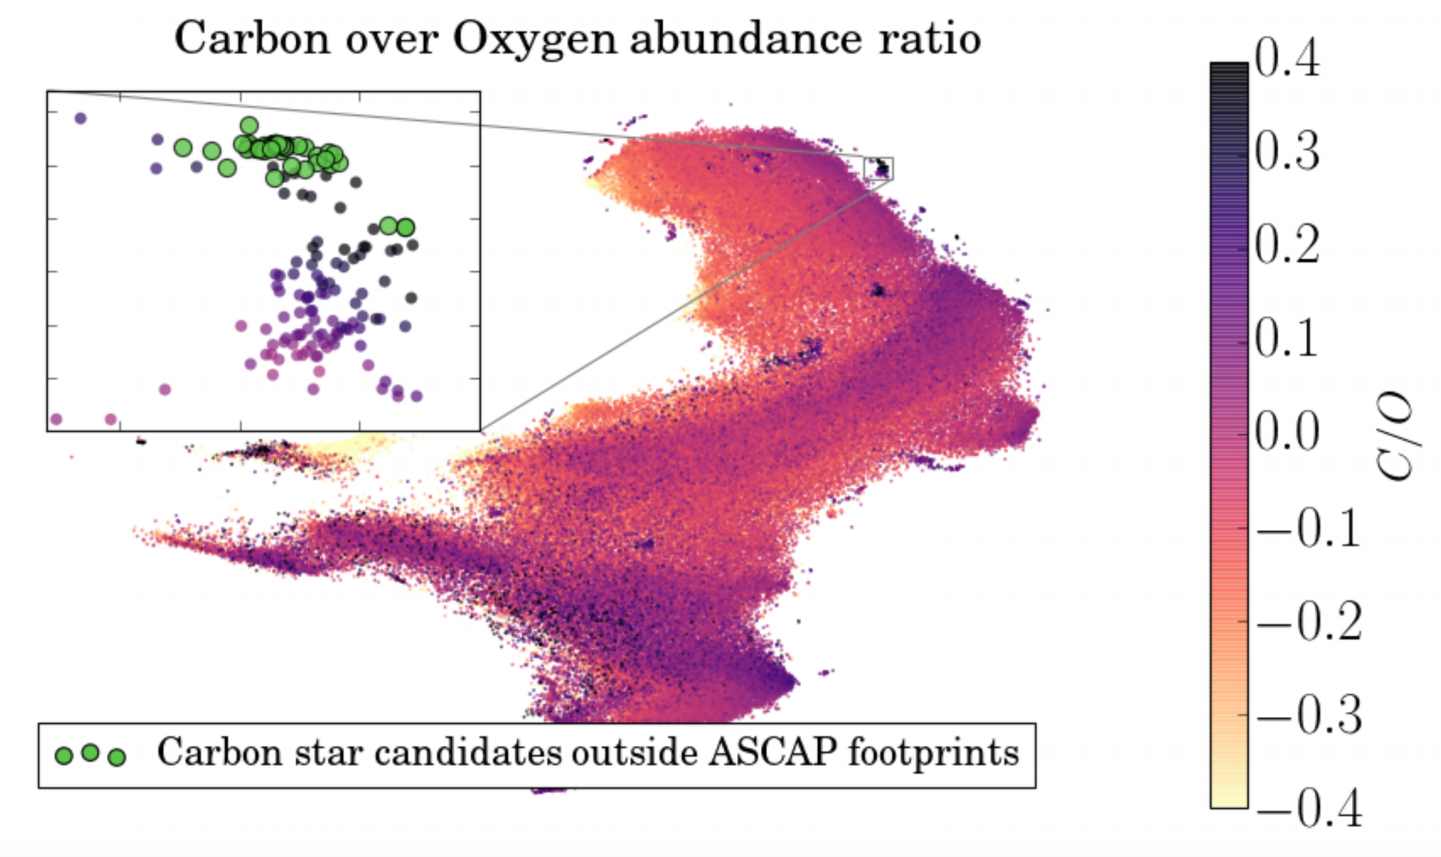
\includegraphics[width=0.8\textwidth]{Images/COar.png} \\ 
Derived-score anomaly detection may help (... or it may not) [Baron]
\end{center}

\newpage
\begin{center}
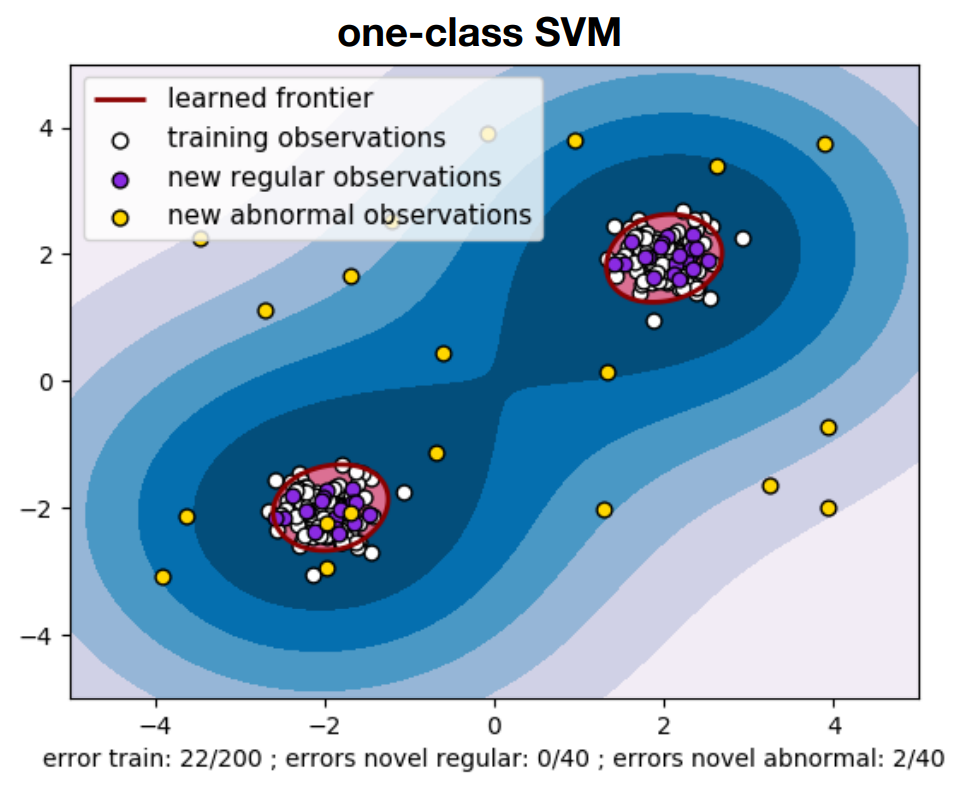
\includegraphics[width=0.68\textwidth]{Images/1SVM.png} \\ 
Learning an \textbf{anomaly frontier} [Baron].
\end{center}


\newpage
\begin{center}
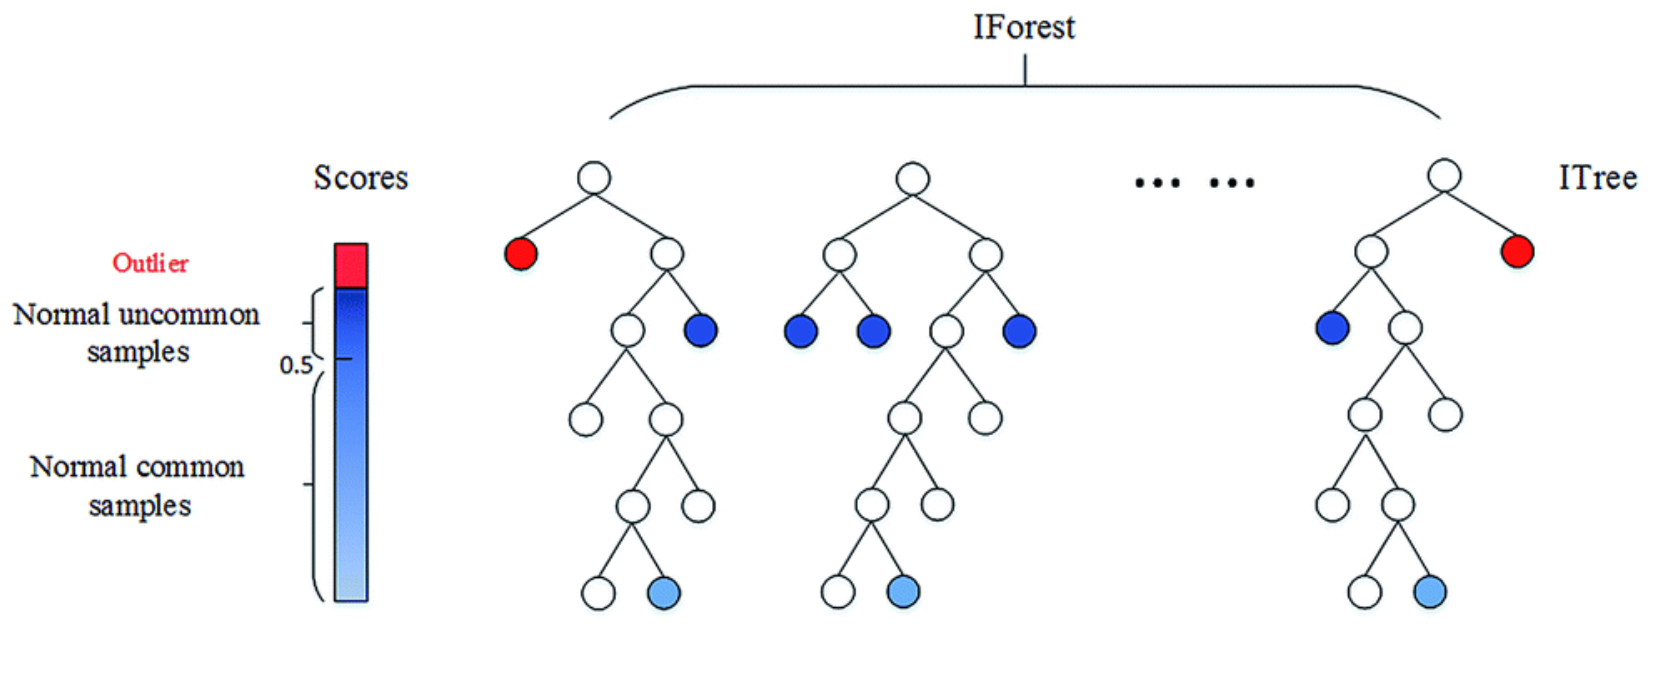
\includegraphics[width=\textwidth]{Images/IsoForest.png} \\ 
\textbf{Isolation Forest:} ensemble method (sections 6.2, 6.6). ``Outliers are objects that are separated from the rest of the dataset higher in the trees'' [Baron, here and next page].
\end{center}

\newpage
\begin{center}
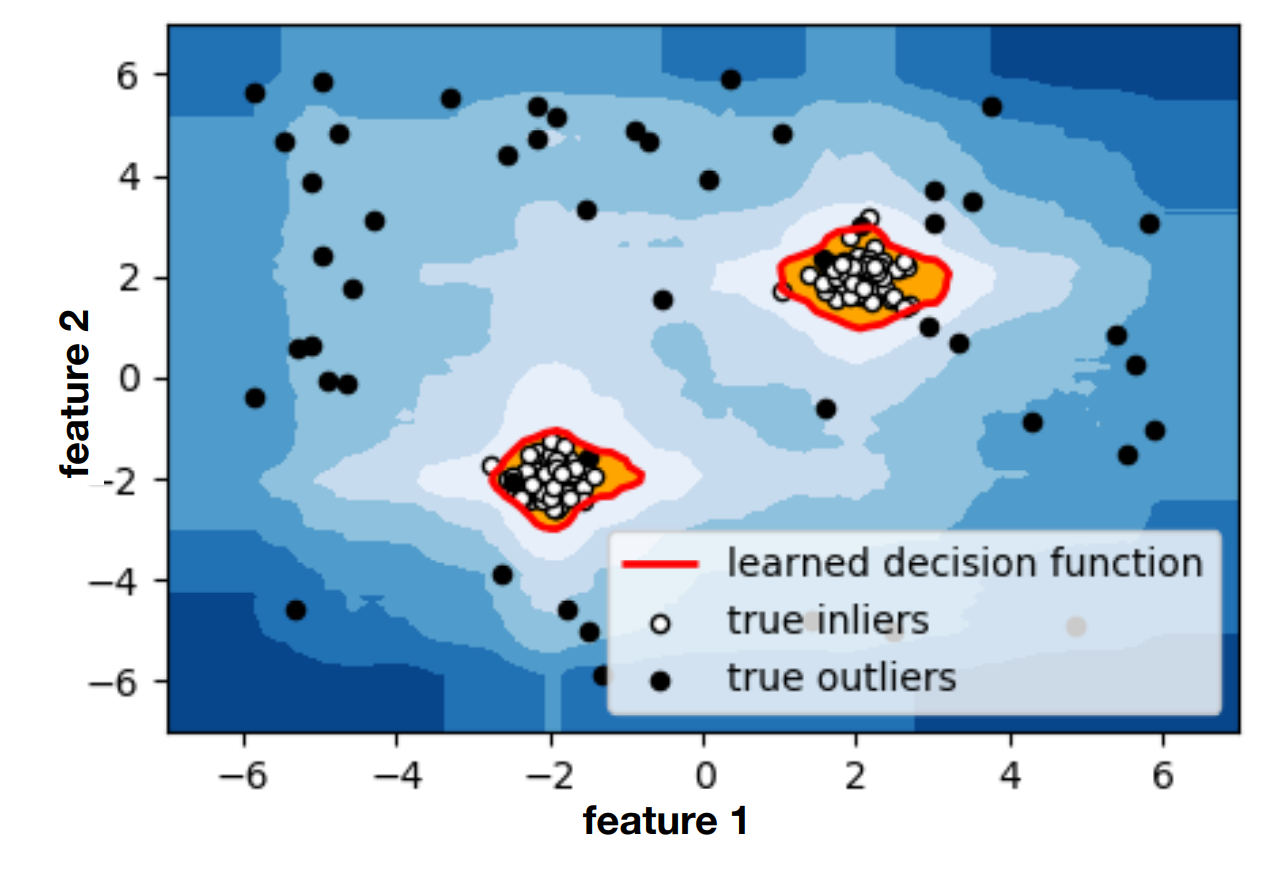
\includegraphics[width=0.9\textwidth]{Images/IsoForest2.png}
\end{center}


\newpage
\begin{center}
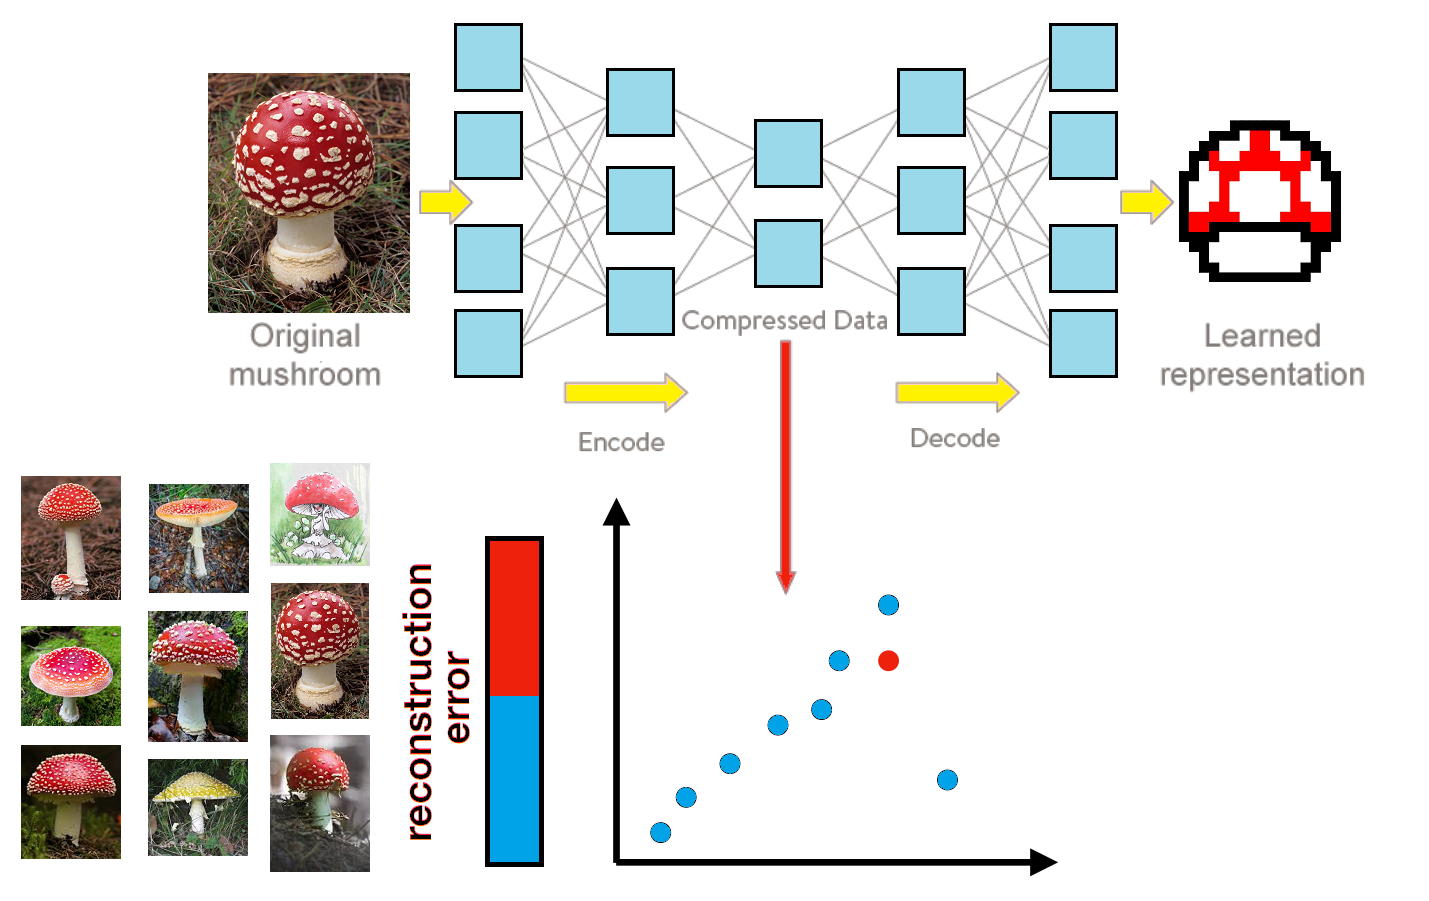
\includegraphics[width=\textwidth]{Images/autoencoder2.png}
\end{center}
\newpage \ \\ \noindent
\noindent \textbf{Autoencoders} learn a compressed representation of the data (dimension reduction).
\newl The \textbf{reconstruction error} measures (in a sense) how much information is lost in the compression. 
\newl Anomaly detection algorithms can be applied to the compressed data:
\begin{itemize}
\item look for anomalous patters, and/or
\item anomalous reconstruction errors. 
\end{itemize}
[Previous slide adapted from Baron].
\newpage\ \\ \noindent
\textbf{Simple analytical methods} using Cooke's or Mahalanobis' distances are sometimes used, but more sophisticated analysis is usually required, especially when trying to identify influential points (\textit{cf.} \textbf{leverage}). 
\newl 
In small datasets, detection can be conducted on a case-by-case basis.\newl \textbf{Questions:} how many anomalies are too many to find? How many cases are you willing to inspect manually? 
\newl It is tempting to use \textbf{automated detection/removal} with large datasets, but doing so may be catastrophic from a data analysis perspective!
\newl If once ``anomalous'' observations have been removed from the dataset, previously ``regular'' observations can become anomalous in turn in the smaller dataset -- when does the runaway train?
\newpage\ \\ 
\begin{center}
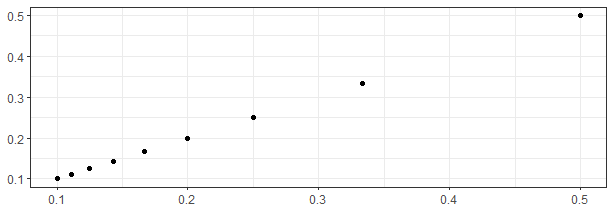
\includegraphics[width=0.45\textwidth]{Images/ADOA1.png}\quad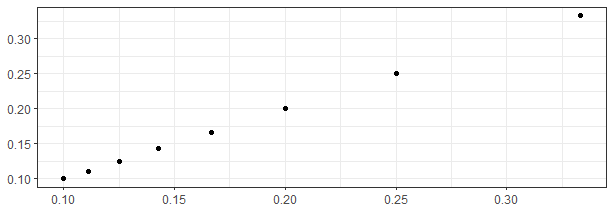
\includegraphics[width=0.45\textwidth]{Images/ADOA2.png} \bigskip
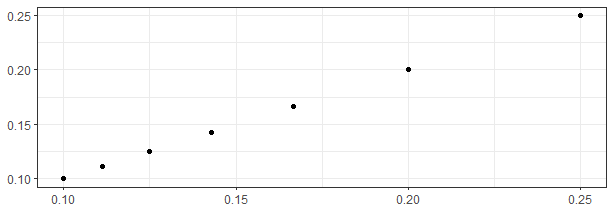
\includegraphics[width=0.45\textwidth]{Images/ADOA3.png}\quad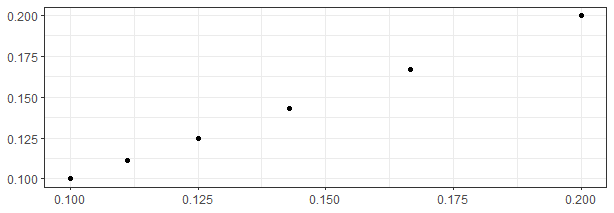
\includegraphics[width=0.45\textwidth]{Images/ADOA4.png} \bigskip
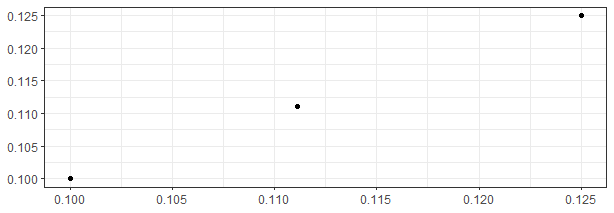
\includegraphics[width=0.45\textwidth]{Images/ADOAn.png}\quad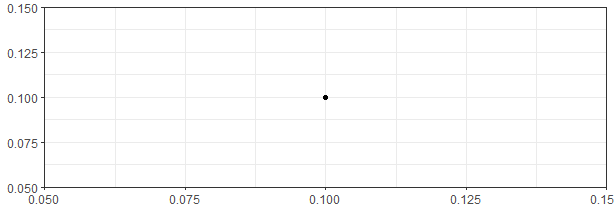
\includegraphics[width=0.45\textwidth]{Images/ADOA10.png}\end{center}

\newpage\ \\ \noindent In the early stages of anomaly detection, we use \textbf{simple data analyses:}
\begin{itemize}
\item descriptive statistics, 
\item $1-$ and $2-$way tables, and  
\item traditional  visualizations.
\end{itemize}
The goal is to \textbf{help identify anomalous observations} and to \textbf{obtain insights about the data}.
\newl 
This leads to more sophisticated anomaly detection methods and could also could eventually lead to modifications of the analysis plan. 
\newl \textbf{THIS IS NEVER AN UNWELCOME DEVELOPMENT!}


\fh{Learning Framework} 
\noindent How are outliers detected, in practice? 
\newl Methods come in two flavours: 
\begin{itemize}
\item \textbf{supervised}, and 
\item \textbf{unsupervised}.\end{itemize}
\textbf{Supervised methods} (SL) use a historical record of \textbf{previously identified anomalous observations} to build a \textbf{predictive classification or regression model} which estimates the probability that a unit is anomalous.
\newpage\ \\ \noindent  \textbf{SL Challenges:} 
\begin{itemize}
\item domain expertise and resources are required to tag the data;
\item since anomalies are typically \textbf{infrequent}, these models often also have to accommodate the \textbf{rare occurrence} (or class imbalance) problem, and 
\item SL methods need to minimize a \textbf{loss function} (cost of making a mistake) which is usually symmetrical (in the anomaly detection context, this  is not usually a valid assumption). 
\end{itemize}
Even more than in traditional analysis settings, anomaly detection can lead to \textbf{technically correct but ultimately useless} (non-actionable) \textbf{results}. 
\newpage\ \\ \noindent  \textbf{Example:} The vast majority ($99.999+$\%) of air passengers \textbf{do not} bring weapons with them on flights. \newl A model that predicts that no passenger is ever attempting to smuggle a weapon on board a flight would be $99.999+$\% accurate.\newl But it would miss the point \textbf{completely}. For the \textbf{security agency}, the cost of wrongly thinking that a passenger is:
\begin{itemize}
\item  smuggling a weapon $\Longrightarrow$ cost of a single search;
\item NOT smuggling a weapon $\Longrightarrow$ catastrophe (potentially). 
\end{itemize}
\noindent The wrongly targeted individuals may have a  ... somewhat different take on this, from a societal and personal perspective.

\newpage\ \\ \noindent \textbf{Unsupervised methods} (UL) \begin{itemize}
\item use no previously labeled (anomalous/non-anomalous) data, and 
\item try to determine if an observation anomalous solely by comparing its behaviour to that of the other observations. 
\end{itemize}
\textbf{Example:} if all workshop participants except for one can view the video conference lectures, then the one individual/internet connection/computer is \textbf{anomalous} -- it behaves in a manner which is different from  the others. \newl 
\textbf{VERY IMPORTANT NOTE:} this \textbf{DOES NOT} mean that the different behaviour is the one we are actually interested in/searching for! 
\newl Be weary: this is true of anomaly detection in data and in real-life. 
\newpage
\begin{center}

\includegraphics[width=0.95\textwidth]{Images/fish.png}
\end{center}

\fh{Traditional Outlier Detection Tests}
\noindent The most commonly-used test is \textbf{Tukey's} (univariate) \textbf{boxplot test}. Let $Q_1$ and $Q_3$ represent an observed feature's $1^{\textrm{st}}$ and $3^{\textrm{rd}}$ quartile, respectively.\newl For \textbf{normally distributed} measurements, regular observations typically lie between the \textbf{inner fences} $$Q_1-1.5(Q_3-Q_1) \quad\mbox{and}\quad Q_3+1.5(Q_3-Q_1).$$ \textbf{Suspected outliers} lie between the inner fences and their \textbf{outer fences} 
$$Q_1-3(Q_3-Q_1) \quad\mbox{and}\quad Q_3+3(Q_3-Q_1).$$
Points beyond the outer fences are identified as \textbf{outliers}. 

\begin{center}
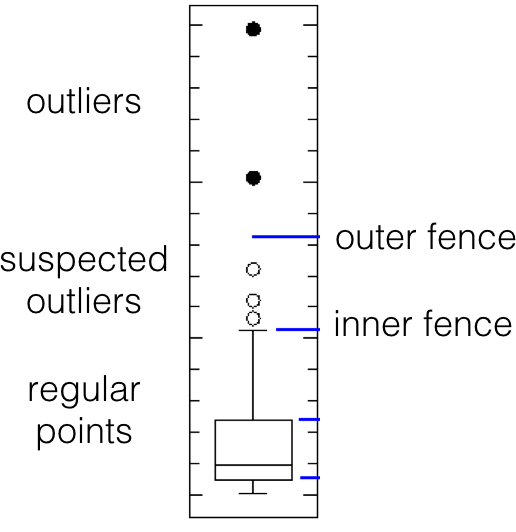
\includegraphics[height=0.8\textheight]{Images/boxplot_EN.png}
\\
Suspected outliers are marked by white disks, outliers by black disks.  \\ Use \texttt{boxplot()} and \texttt{boxplot.stats()} in \texttt{R} to plot and identify outliers in normally distributed data.
\end{center}
\newpage\ \\ \noindent The \textbf{Grubbs test} is another univariate test: 
$$H_0: \text{ no outlier in the data vs.\@ } H_1: \text{ \textbf{exactly one} outlier in the data.}$$

%, which takes into consideration the \textbf{number of observations} in the dataset:
\begin{itemize}
\item let $x_i$ be the value of feature $X$ for the $i^{\textrm{th}}$ unit, $1\leq i\leq N$,\item  let $(\overline{x},s_x)$ be the mean and standard deviation of feature $X$, 
\item let $\alpha$ be the desired significance level, and 
\item let  $T(\alpha/2N;N)$ be the critical value of the Student $t$-distribution. 
\end{itemize} 
The test statistic is $$G=\frac{\max_i\{|x_i-\overline{x}|\}}{s_x}=\frac{|x_{i^*}-\overline{x}|}{s_x}.$$

\newpage\ \\ \noindent Under $H_0$, $G$ follows a special distribution with critical value $$\ell(\alpha;N)=\frac{N-1}{\sqrt{N}}\sqrt{\frac{T^2(\alpha/2N,N)}{N-2+T^2(\alpha/2N,N)}}.$$ 
At significance level $\alpha$, we reject the null hypothesis in favour of the alternative (i.e.\@ $x_{i^*}$ is the outlier) if  $G\geq \ell(\alpha;N)$.
\newl If looking for more than one outlier, it can be tempting to classify every observation $i$ for which 
$$\frac{|x_i-\overline{x}|}{s_x} \geq \ell(\alpha;N)$$ as an outlier, but this is \textbf{NOT RECOMMENDED}. 
\newl Other generalizations are also problematic (cf.\@ outlier sequence). 

\newpage\ \\ \noindent Other common tests include:
\begin{itemize}

\item the \textbf{Mahalanobis distance}, which is linked to the leverage of an observation (a measure of influence), can also be used to find multi-dimen\-sio\-nal outliers, when all relationships are linear (or nearly linear);

\item the \textbf{Tietjen-Moore} test, which is used to find a specific number of outliers (this is similar to Grubbs' test, replacing $H_1$ by $H_k$);

\item the \textbf{generalized extreme studentized deviate} test, the preferred extension to Grubbs' test if the number of outliers is unknown; 

\item the \textbf{chi-square} test, when outliers affect the goodness-of-fit;

\item DBSCAN and other clustering-based outlier detection methods.

\end{itemize}



\fh{Visual Outlier Detection} 
\normalsize
\noindent The following simple examples illustrate the principles underlying \textbf{visual outlier and anomaly detection}. 

\noindent \textbf{Example 1:} on a specific day, the \textbf{height} of several plants in a nursery are measured. The records also show each plant's \textbf{age} (the number of weeks since the seed has been planted). 
\newl Very little can be said about the data at that stage: 
\begin{itemize}
\item the age of the plants (controlled by the nursery staff) seems to be somewhat haphazard, 
\item as does the response variable (height). 
\end{itemize}
\newpage\ 
\begin{center}
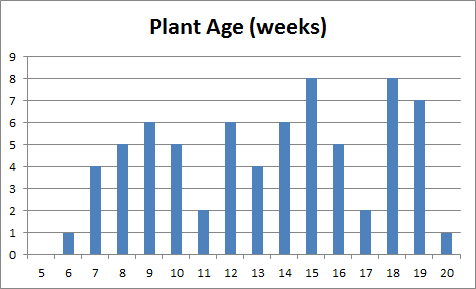
\includegraphics[width=0.47\textwidth]{Images/plant_age_EN}\\ 
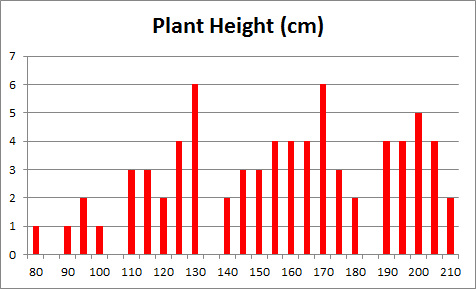
\includegraphics[width=0.47\textwidth]{Images/plant_height_EN}
\end{center}
\newpage\ \\ \noindent A scatter plot of the data reveals that \textbf{growth is strongly correlated with age} for the observations in the dataset; points clutter around a linear trend. \newl One point (in yellow) is easily identified as an \textbf{outlier}. \newl There are (at least) two possibilities: 
\begin{itemize}
\item either that measurement was botched or mis-entered in the database (representing an invalid entry), or 
\item that one specimen has experienced unusual growth (outlier).
\end{itemize}
Either way, the analyst has to investigate further.
\newpage\ 
\begin{center}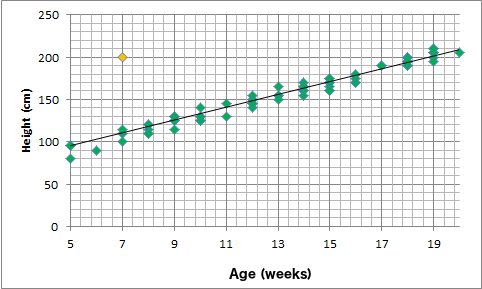
\includegraphics[width=0.90\textwidth]{Images/plant_height_vs_age_EN}\end{center} 
\newpage\ \\ \noindent \textbf{Example 2:} 
a government department has 11 service points. The monthly average arrival and service rates per teller for each service point are available. \newl The scatter plot of the service rate per teller ($y$ axis) against the arrival rate per teller ($x$ axis), with linear regression trend, is shown below. 

\begin{center}
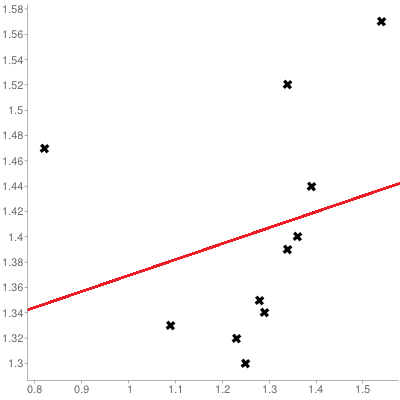
\includegraphics[width=0.37\textwidth]{Images/scatter_plot_linear_1}
\end{center}
\newpage\ \\ \noindent 
A similar chart, but with the left-most point removed from consideration, is shown below. 
\begin{center}
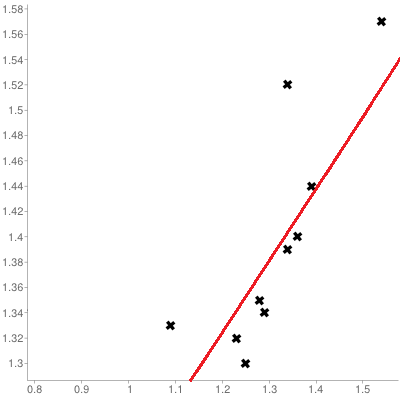
\includegraphics[width=0.37\textwidth]{Images/scatter_plot_linear_2}
\end{center}
The trend still slopes upward, but the fit is significantly improved. \newpage\ \\ \noindent This suggests that the removed observation is unduly \textbf{influential} (or anomalous) -- a better understanding of the relationship between arrivals and services is afforded if it is set aside. 
\newl Any attempt to fit that data point into the model must take this information into consideration. \newl The status of an influential observations \textbf{depends on the analysis that is ultimately conducted} -- a point may be influential for one analysis, but not for another. 
\newl Note that setting aside an influential observation does not mean that the observation is removed from the dataset -- only that it will not be used in a specific analysis. 
\newpage\ \\ \noindent \textbf{Example 3:} Measurements of the length of the appendage of a certain species of insect have been made on 71 individuals. Descriptive statistics have been computed; the results are shown below.
\begin{center}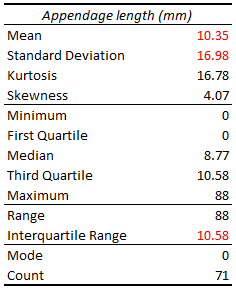
\includegraphics[height=0.72\textheight]{Images/appendage_length_descriptive_EN}
\end{center}  

\newpage\ \\ \noindent The descriptive statistics might help the analyst recognize the tell-tale signs that the distribution of appendage lengths is likely to: \begin{itemize}
\item be \textbf{asymmetrical} (since skewness is non-negligible), and
\item have a \textbf{``fat'' tail} (since large kurtosis, range $\gg$ interquartile range, and max $\gg Q_3$) \end{itemize} 
The mode, min, and $Q_1$ belong to individuals without appendages $\Longrightarrow$ at least two sub-groups in the population (perhaps split along the lines of juveniles/adults, or males/females).\newl Since max $\gg$ other observations, might it  belong to an \textbf{outlier}? The histogram of the measurements shows 3 individuals with long appendages.\newpage\ 
\begin{center} 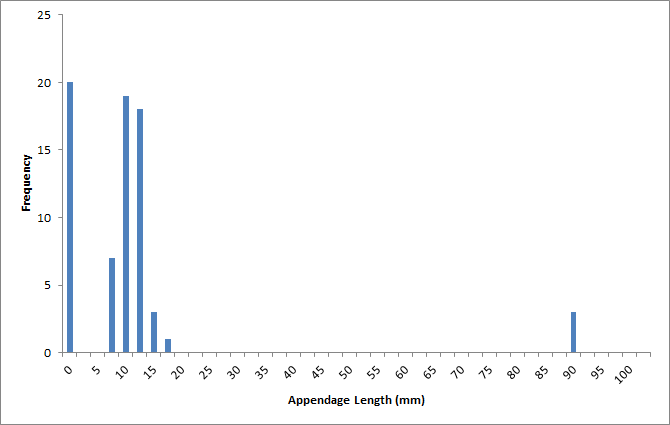
\includegraphics[width=0.9\textwidth]{Images/appendage_length_EN}
\end{center}  
\newpage \ \\ \noindent
It is plausible that these individuals belong to another species who were \textbf{erroneously added} to the dataset. \newl On its own, the chart does not constitute a proof of such an error, but it \textbf{raises the possibility of an error}, which is often the best that an analyst can do in the absence of subject matter expertise.
\newl This traditional approach to anomaly detection is difficult to apply to high-dimensional datasets because it is nearly impossible to visualize them directly $\Longrightarrow$ fundamentally different approaches are needed.\newl 
Dimension reduction methods can be used to provide a \textbf{low-dimensional representation} of the data on which to apply visual detection (see autoencoder example), but some information always gets lost in the process. 

\fh{6.1.1 -- Anomaly Detection as Statistical Learning} \label{6.1.1} 
\noindent Fraudulent behaviour is not always easily identifiable, even after the fact. \newl \textbf{Example:} credit card fraudsters try to disguise their transactions as regular and banal, and try to avoid outlandish behaviour. \newl Their goal: fool human observers into confusing  \textbf{plausible} (or possible) with \textbf{probable} (or at least, \textbf{not improbable}). \newl It is plausible that a generic 40-something father of 3 might purchase a new TV; is it probable that THIS particular father of 3  would do so? \newl But it's unlikely that a generic father of 3 who resides in North America would purchase a round of drinks at a dance club in Kiev. \newpage\ \\ \noindent Anomaly detection is really a problem in \textbf{applied probability}. Let $I$ be what is known about the dataset/situation: 
\begin{itemize}
\item behaviour of individual observations,
\item behaviour of observations as a whole, 
\item anomalous/normal verdict for a number of similar observations, etc.
\end{itemize} \textbf{Main Question:} is $P(\text{obs.\@ is anomalous}\mid I) > P(\text{obs.\@ is normal}\mid I)?$ 
\newl Anomaly detection models assume \textbf{stationarity of regular observations}: that the underlying mechanism that generates regular data does not change much over time.\newpage \ \\ \noindent For time series data, this means that it may be necessary to first perform \textbf{trend and seasonality extraction}.\newl 
\textbf{Example:} supply chains play a crucial role in the transportation of goods from one part of the world to another -- as the saying goes, ``a given chain is only as strong as its weakest link.'' \newl Say that marine cargo departing Shanghai in Feb'13 took two more days, on average, to arrive in Vancouver than those departing in Jul'17.
\begin{itemize}
\item Has the shipping process  improved in the intervening years? 
\item Do departures in Feb usually take longer to reach Vancouver? 
\item Are either the Feb'13 or the Jul'17 performance anomalous?
\end{itemize} \newpage\ \\ \noindent Seasonal variability is relevant to supply chain monitoring: quantifying and accounting for impact severity is of great interest. \newl  
\textbf{Potential Solution:} create an \textbf{index} to track container transit times. \newl This index should depict 
\begin{itemize}
\item \textbf{reliability} and
\item \textbf{variability} of transit times, 
\item and allow for performance comparison between differing time periods.
\end{itemize} 
\newpage\ \\ \noindent Consider the scenario where we want to compare the  monthly performance, irrespective of the transit season, of the corridor $$\textbf{Shanghai} \to \textbf{Port Metro Vancouver/Prince Rupert} \to \textbf{Toronto}.$$  
\begin{center}
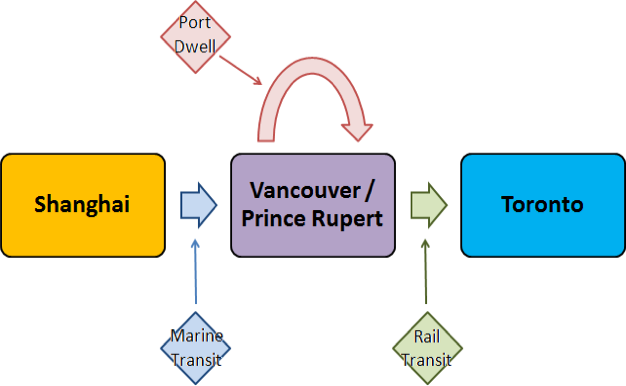
\includegraphics[width=0.65\textwidth]{Images/mmsc_EN.png}
\end{center}
\newpage\ \\ \noindent 
For each of the three segments (Marine Transit, Port Dwell, Rail Transit), the data consists of:
\begin{itemize}
\item monthly empirical distribution of transit/dwell times
\item built from sub-samples (assumed to be randomly selected and fully representative) of all containers entering the appropriate segment.
\end{itemize}
Specific containers are not followed from Shanghai to Toronto: no covariance information about the various transit/dwell times is available. \newl Each segment's performance is measured using \textbf{fluidity indicators}, which are computed using various statistics of the transit/dwell time distributions for each of the supply chain segments. 
\newpage\ \begin{description} 
\item[Reliability Indicator (RI)] -- the ratio of the 95$^{\text{th}}$ percentile to the 5$^{\text{th}}$ percentile of transit/dwell times. \par A high RI indicates high volatility, whereas a low RI $(\approx 1)$ indicates a reliable corridor.
\item[Buffer Index (BI)] -- the ratio of the positive difference between the 95$^{\text{th}}$ percentile and the mean, to the mean. \par A small BI $(\approx 0)$ indicates only slight variability in the upper (longer) transit/dwell times; a large BI indicates that the variability of the longer transit/dwell times is high, and that outliers might be found there;
\item[Coefficient of Variation (CV)] -- the ratio of the standard deviation of transit/dwell times to the mean transit/dwell time.  
\end{description}
\newpage\ \\ 
\begin{center}
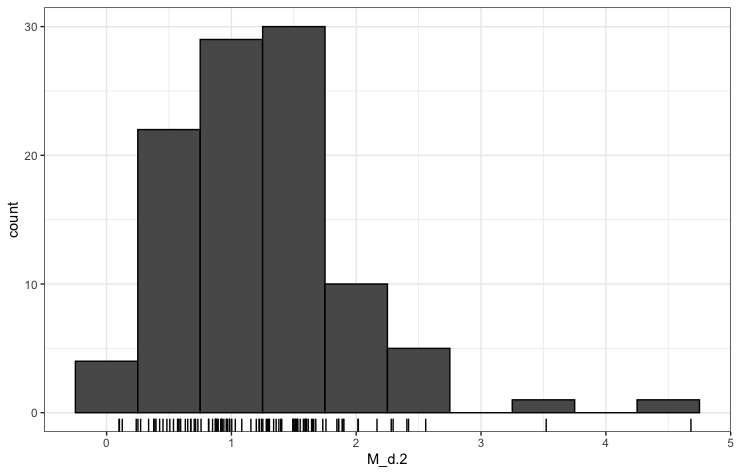
\includegraphics[width=\textwidth]{Images/Rplot}
\\
%\begin{threeparttable}
 \setlength{\tabcolsep}{1pt}
\begin{tabularx}{\textwidth}{p{0.1\textwidth} p{0.1\textwidth} p{0.1\textwidth} p{0.1\textwidth} p{0.1\textwidth} p{0.1\textwidth} p{0.1\textwidth} p{0.1\textwidth} p{0.1\textwidth}}


\hhline{}
\arrayrulecolor{black}

\multicolumn{1}{!{\huxvb{0, 0, 0}{0}}p{0.1\textwidth}!{\huxvb{0, 0, 0}{0}}}{\hspace{0pt}\parbox[b]{0.1\textwidth-10pt-10pt}{\huxtpad{6pt + 1em}\raggedright \textbf{Segmt}\huxbpad{6pt}}} &
\multicolumn{1}{p{0.1\textwidth}!{\huxvb{0, 0, 0}{0}}}{\hspace{10pt}\parbox[b]{0.1\textwidth-10pt-10pt}{\huxtpad{6pt + 1em}\raggedleft \textbf{Freq}\huxbpad{6pt}}} &
\multicolumn{1}{p{0.1\textwidth}!{\huxvb{0, 0, 0}{0}}}{\hspace{10pt}\parbox[b]{0.1\textwidth-10pt-10pt}{\huxtpad{6pt + 1em}\raggedleft \textbf{Mean}\huxbpad{6pt}}} &
\multicolumn{1}{p{0.1\textwidth}!{\huxvb{0, 0, 0}{0}}}{\hspace{10pt}\parbox[b]{0.1\textwidth-10pt-10pt}{\huxtpad{6pt + 1em}\raggedleft \textbf{SD}\huxbpad{6pt}}} &
\multicolumn{1}{p{0.1\textwidth}!{\huxvb{0, 0, 0}{0}}}{\hspace{10pt}\parbox[b]{0.1\textwidth-10pt-10pt}{\huxtpad{6pt + 1em}\raggedleft \textbf{C05}\huxbpad{6pt}}} &
\multicolumn{1}{p{0.1\textwidth}!{\huxvb{0, 0, 0}{0}}}{\hspace{10pt}\parbox[b]{0.1\textwidth-10pt-10pt}{\huxtpad{6pt + 1em}\raggedleft \textbf{C95}\huxbpad{6pt}}} &
\multicolumn{1}{p{0.1\textwidth}!{\huxvb{0, 0, 0}{0}}}{\hspace{10pt}\parbox[b]{0.1\textwidth-10pt-10pt}{\huxtpad{6pt + 1em}\raggedleft \textbf{RI}\huxbpad{6pt}}} &
\multicolumn{1}{p{0.1\textwidth}!{\huxvb{0, 0, 0}{0}}}{\hspace{10pt}\parbox[b]{0.1\textwidth-10pt-10pt}{\huxtpad{6pt + 1em}\raggedleft \textbf{BI}\huxbpad{6pt}}} &
\multicolumn{1}{p{0.1\textwidth}!{\huxvb{0, 0, 0}{0}}}{\hspace{10pt}\parbox[b]{0.1\textwidth-10pt-10pt}{\huxtpad{6pt + 1em}\raggedleft \textbf{CV}\huxbpad{6pt}}} \tabularnewline[-0.5pt]


\hhline{>{\huxb{0, 0, 0}{0.4}}->{\huxb{0, 0, 0}{0.4}}->{\huxb{0, 0, 0}{0.4}}->{\huxb{0, 0, 0}{0.4}}->{\huxb{0, 0, 0}{0.4}}->{\huxb{0, 0, 0}{0.4}}->{\huxb{0, 0, 0}{0.4}}->{\huxb{0, 0, 0}{0.4}}->{\huxb{0, 0, 0}{0.4}}-}
\arrayrulecolor{black}

\multicolumn{1}{!{\huxvb{0, 0, 0}{0}}p{0.1\textwidth}!{\huxvb{0, 0, 0}{0}}}{\hspace{10pt}\parbox[b]{0.1\textwidth-10pt-10pt}{\huxtpad{6pt + 1em}\raggedright $A$\huxbpad{6pt}}} &
\multicolumn{1}{p{0.1\textwidth}!{\huxvb{0, 0, 0}{0}}}{\hspace{10pt}\parbox[b]{0.1\textwidth-10pt-10pt}{\huxtpad{6pt + 1em}\raggedleft 3286\huxbpad{6pt}}} &
\multicolumn{1}{p{0.1\textwidth}!{\huxvb{0, 0, 0}{0}}}{\hspace{10pt}\parbox[b]{0.1\textwidth-10pt-10pt}{\huxtpad{6pt + 1em}\raggedleft 12.10\huxbpad{6pt}}} &
\multicolumn{1}{p{0.1\textwidth}!{\huxvb{0, 0, 0}{0}}}{\hspace{10pt}\parbox[b]{0.1\textwidth-10pt-10pt}{\huxtpad{6pt + 1em}\raggedleft 3.33\huxbpad{6pt}}} &
\multicolumn{1}{p{0.1\textwidth}!{\huxvb{0, 0, 0}{0}}}{\hspace{10pt}\parbox[b]{0.1\textwidth-10pt-10pt}{\huxtpad{6pt + 1em}\raggedleft 7.06\huxbpad{6pt}}} &
\multicolumn{1}{p{0.1\textwidth}!{\huxvb{0, 0, 0}{0}}}{\hspace{10pt}\parbox[b]{0.1\textwidth-10pt-10pt}{\huxtpad{6pt + 1em}\raggedleft 17.00\huxbpad{6pt}}} &
\multicolumn{1}{p{0.1\textwidth}!{\huxvb{0, 0, 0}{0}}}{\hspace{10pt}\parbox[b]{0.1\textwidth-10pt-10pt}{\huxtpad{6pt + 1em}\raggedleft 2.41\huxbpad{6pt}}} &
\multicolumn{1}{p{0.1\textwidth}!{\huxvb{0, 0, 0}{0}}}{\hspace{10pt}\parbox[b]{0.1\textwidth-10pt-10pt}{\huxtpad{6pt + 1em}\raggedleft 0.41\huxbpad{6pt}}} &
\multicolumn{1}{p{0.1\textwidth}!{\huxvb{0, 0, 0}{0}}}{\hspace{10pt}\parbox[b]{0.1\textwidth-10pt-10pt}{\huxtpad{6pt + 1em}\raggedleft 0.27\huxbpad{6pt}}} \tabularnewline[-0.5pt]


\hhline{}
\arrayrulecolor{black}

\multicolumn{1}{!{\huxvb{0, 0, 0}{0}}p{0.1\textwidth}!{\huxvb{0, 0, 0}{0}}}{\hspace{10pt}\parbox[b]{0.1\textwidth-10pt-10pt}{\huxtpad{6pt + 1em}\raggedright $B$\huxbpad{6pt}}} &
\multicolumn{1}{p{0.1\textwidth}!{\huxvb{0, 0, 0}{0}}}{\hspace{10pt}\parbox[b]{0.1\textwidth-10pt-10pt}{\huxtpad{6pt + 1em}\raggedleft 2594\huxbpad{6pt}}} &
\multicolumn{1}{p{0.1\textwidth}!{\huxvb{0, 0, 0}{0}}}{\hspace{10pt}\parbox[b]{0.1\textwidth-10pt-10pt}{\huxtpad{6pt + 1em}\raggedleft 10.09\huxbpad{6pt}}} &
\multicolumn{1}{p{0.1\textwidth}!{\huxvb{0, 0, 0}{0}}}{\hspace{10pt}\parbox[b]{0.1\textwidth-10pt-10pt}{\huxtpad{6pt + 1em}\raggedleft 4.43\huxbpad{6pt}}} &
\multicolumn{1}{p{0.1\textwidth}!{\huxvb{0, 0, 0}{0}}}{\hspace{10pt}\parbox[b]{0.1\textwidth-10pt-10pt}{\huxtpad{6pt + 1em}\raggedleft 3.88\huxbpad{6pt}}} &
\multicolumn{1}{p{0.1\textwidth}!{\huxvb{0, 0, 0}{0}}}{\hspace{10pt}\parbox[b]{0.1\textwidth-10pt-10pt}{\huxtpad{6pt + 1em}\raggedleft 18.20\huxbpad{6pt}}} &
\multicolumn{1}{p{0.1\textwidth}!{\huxvb{0, 0, 0}{0}}}{\hspace{10pt}\parbox[b]{0.1\textwidth-10pt-10pt}{\huxtpad{6pt + 1em}\raggedleft 4.69\huxbpad{6pt}}} &
\multicolumn{1}{p{0.1\textwidth}!{\huxvb{0, 0, 0}{0}}}{\hspace{10pt}\parbox[b]{0.1\textwidth-10pt-10pt}{\huxtpad{6pt + 1em}\raggedleft 0.80\huxbpad{6pt}}} &
\multicolumn{1}{p{0.1\textwidth}!{\huxvb{0, 0, 0}{0}}}{\hspace{10pt}\parbox[b]{0.1\textwidth-10pt-10pt}{\huxtpad{6pt + 1em}\raggedleft 0.44\huxbpad{6pt}}} \tabularnewline[-0.5pt]


\hhline{}
\arrayrulecolor{black}

\multicolumn{1}{!{\huxvb{0, 0, 0}{0}}p{0.1\textwidth}!{\huxvb{0, 0, 0}{0}}}{\hspace{10pt}\parbox[b]{0.1\textwidth-10pt-10pt}{\huxtpad{6pt + 1em}\raggedright $C$\huxbpad{6pt}}} &
\multicolumn{1}{p{0.1\textwidth}!{\huxvb{0, 0, 0}{0}}}{\hspace{10pt}\parbox[b]{0.1\textwidth-10pt-10pt}{\huxtpad{6pt + 1em}\raggedleft 2142\huxbpad{6pt}}} &
\multicolumn{1}{p{0.1\textwidth}!{\huxvb{0, 0, 0}{0}}}{\hspace{10pt}\parbox[b]{0.1\textwidth-10pt-10pt}{\huxtpad{6pt + 1em}\raggedleft 5.96\huxbpad{6pt}}} &
\multicolumn{1}{p{0.1\textwidth}!{\huxvb{0, 0, 0}{0}}}{\hspace{10pt}\parbox[b]{0.1\textwidth-10pt-10pt}{\huxtpad{6pt + 1em}\raggedleft 5.08\huxbpad{6pt}}} &
\multicolumn{1}{p{0.1\textwidth}!{\huxvb{0, 0, 0}{0}}}{\hspace{10pt}\parbox[b]{0.1\textwidth-10pt-10pt}{\huxtpad{6pt + 1em}\raggedleft 0.19\huxbpad{6pt}}} &
\multicolumn{1}{p{0.1\textwidth}!{\huxvb{0, 0, 0}{0}}}{\hspace{10pt}\parbox[b]{0.1\textwidth-10pt-10pt}{\huxtpad{6pt + 1em}\raggedleft 14.40\huxbpad{6pt}}} &
\multicolumn{1}{p{0.1\textwidth}!{\huxvb{0, 0, 0}{0}}}{\hspace{10pt}\parbox[b]{0.1\textwidth-10pt-10pt}{\huxtpad{6pt + 1em}\raggedleft 77.12\huxbpad{6pt}}} &
\multicolumn{1}{p{0.1\textwidth}!{\huxvb{0, 0, 0}{0}}}{\hspace{10pt}\parbox[b]{0.1\textwidth-10pt-10pt}{\huxtpad{6pt + 1em}\raggedleft 1.41\huxbpad{6pt}}} &
\multicolumn{1}{p{0.1\textwidth}!{\huxvb{0, 0, 0}{0}}}{\hspace{10pt}\parbox[b]{0.1\textwidth-10pt-10pt}{\huxtpad{6pt + 1em}\raggedleft 0.85\huxbpad{6pt}}} \tabularnewline[-0.5pt]


\hhline{}
\arrayrulecolor{black}
\end{tabularx} \end{center}
\newpage\ \\ \noindent The time series of monthly fluidity indicators  are then \textbf{decomposed} into: 
\begin{itemize} 
\item trend $\Longrightarrow$ \textbf{expected behaviour}
\item seasonal component (seasonality, trading-day, moving-holiday) $\Longrightarrow$ \textbf{expected behaviour} 
\item structural breaks, $\Longrightarrow$ \textbf{explained unexpected behaviour} and 
\item irregular component $\Longrightarrow$ chain \textbf{volatility}
\end{itemize}
A high irregular component at a given time indicates a poor performance against expectations $\Longrightarrow$ an \textbf{anomalous observation}.  
\newpage
\begin{center}
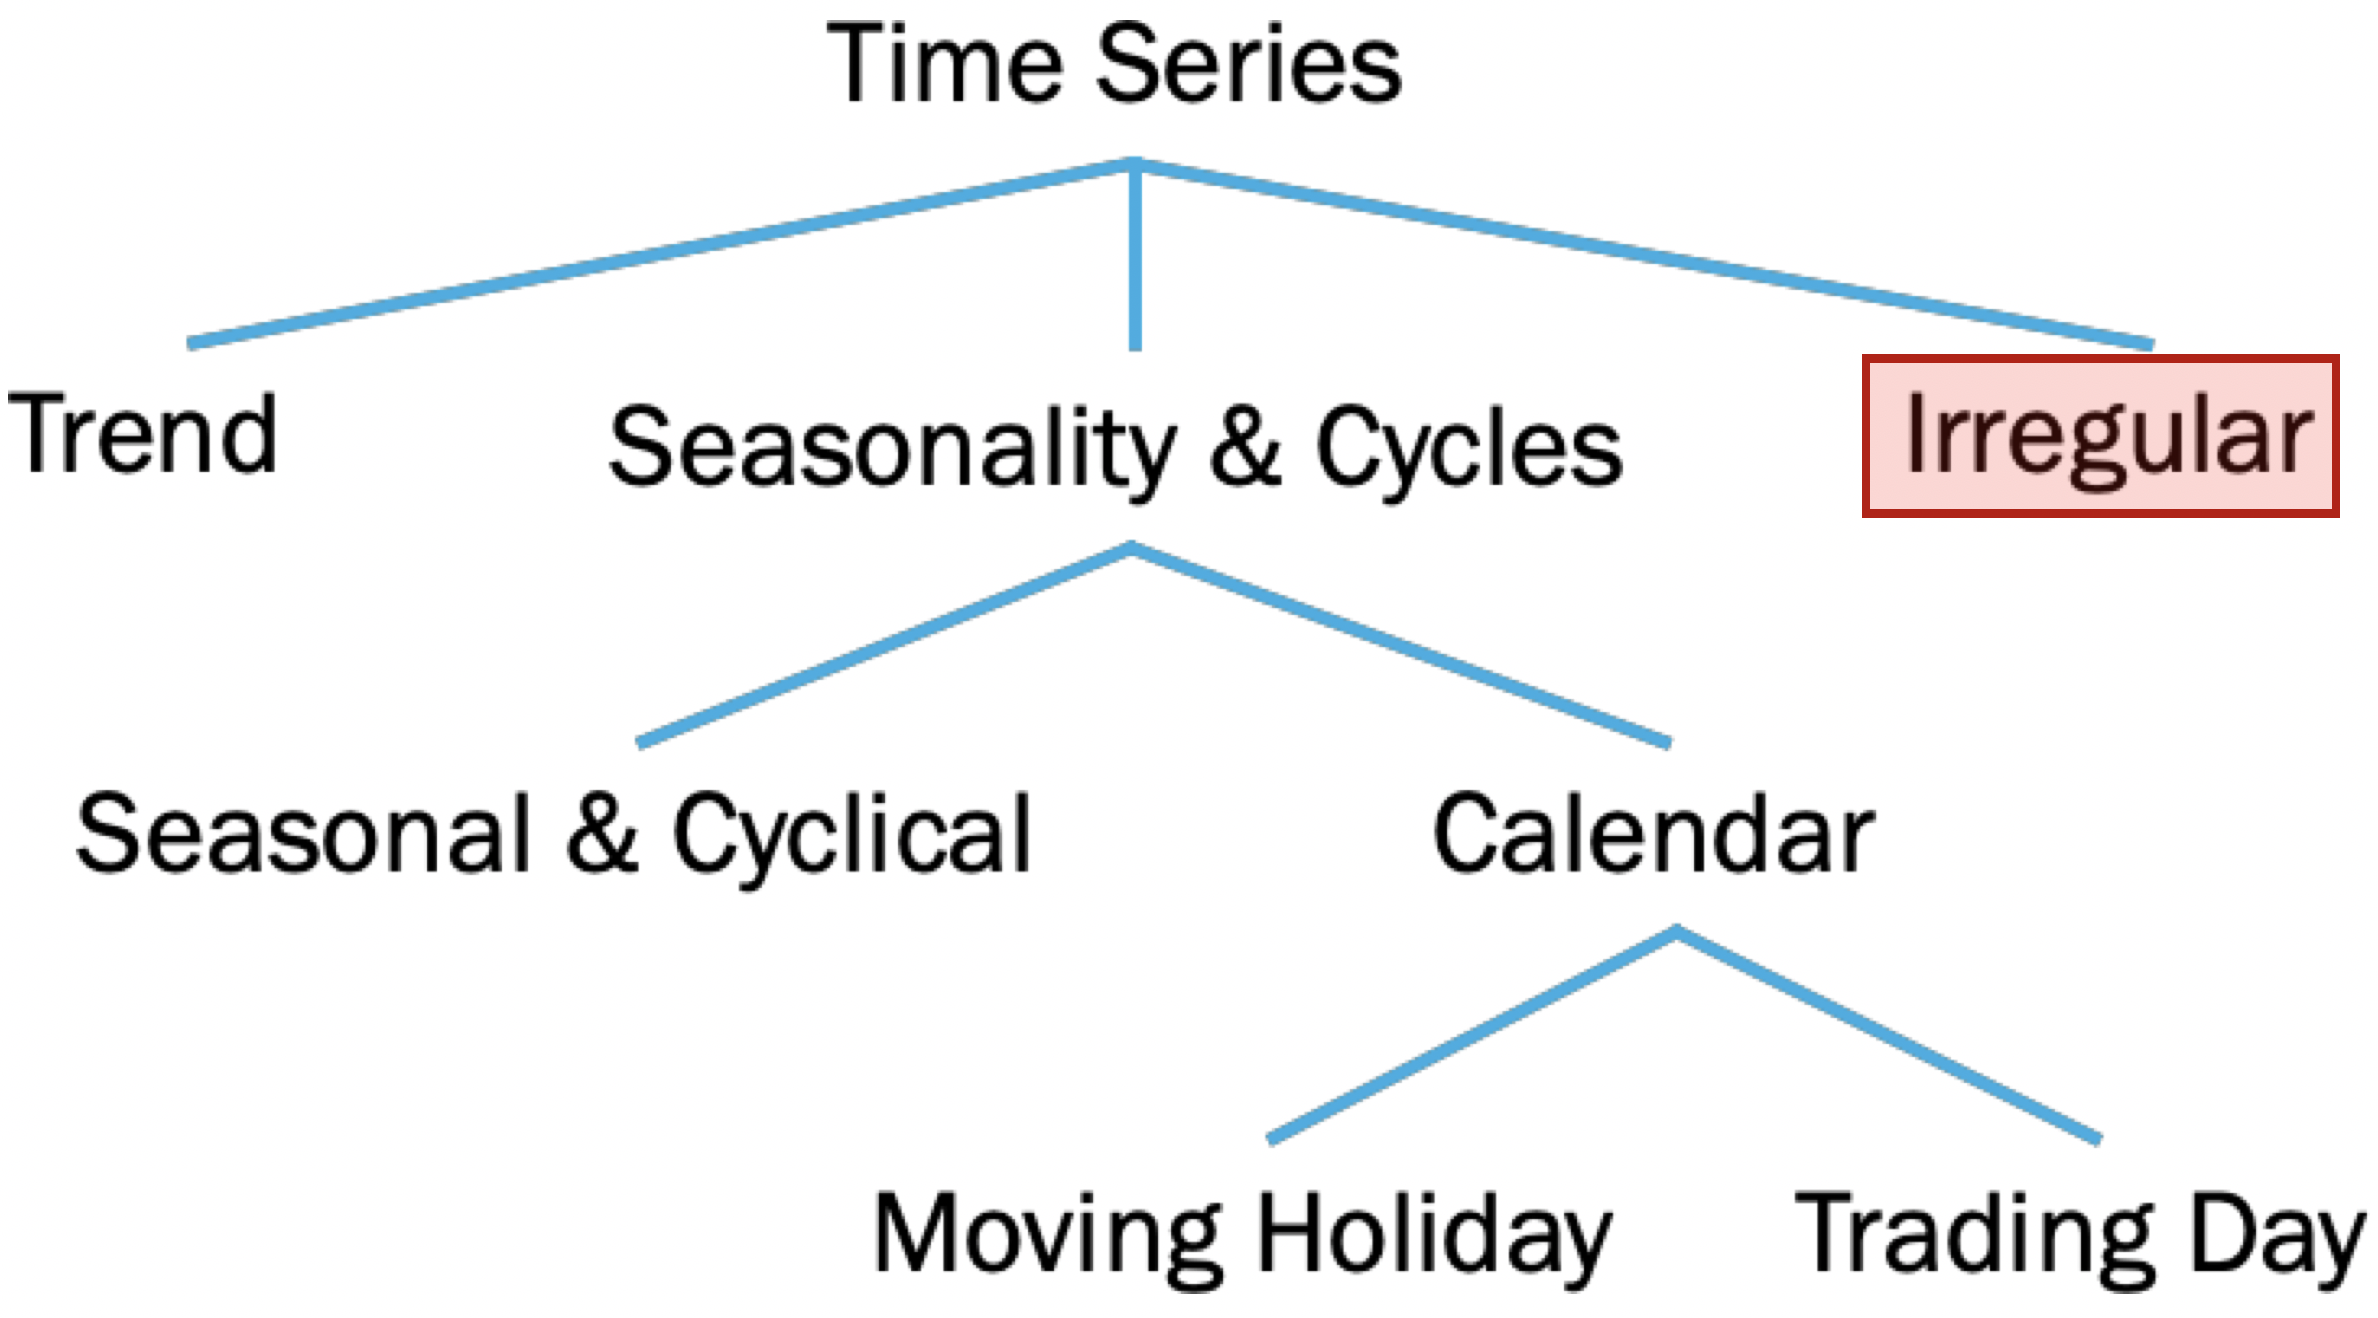
\includegraphics[width=0.85\textwidth]{Images/decomposition_EN.png} \end{center} 
Conceptual time series decomposition (after structural breaks are removed); potential anomalous behaviour should be searched for in the \textbf{irregular component}.
\newpage\ \\ \noindent In general, the decomposition follows a model which is 
\begin{itemize} 
\item multiplicative;
\item additive, or 
\item pseudo-additive.
\end{itemize}
The choice of a model is driven by data behaviour and choice of assumptions; the X12 model automates some of the aspects of the decomposition, but manual intervention and diagnostics are still required.\newl
\textbf{IMPORTANT NOTE:} anomaly detection often requires modeling choices/ assumptions. 
\newpage\ \\ \noindent 
The \textbf{additive model}, for instance, assumes that: 
\begin{enumerate} \item the seasonal component $S_t$ and the irregular component $I_t$ are independent of the trend $T_t$; \item  the seasonal component $S_t$ remains stable from year to year; and \item there is no seasonal fluctuation: $\sum_{j=1}^{12} S_{t+j}=0 $.\end{enumerate} 
Mathematically, the model is expressed as:
    \begin{equation*}
        O_t = T_t + S_t + I_t
    \end{equation*}
    All components share the same dimensions and units. \newpage\ \\ \noindent After seasonality adjustment,the seasonality adjusted series is:
    \begin{equation*}
        SA_t = O_t - S_t = T_t + I_t
    \end{equation*}
The multiplicative and pseudo-additive models are defined in similar ways:\begin{itemize} 
\item if the size of $S_t$   increases/decreases over time, use s multiplicative model; 
\item otherwise, use an additive model.
\end{itemize}
The data decomposition/preparation process is illustrated with the 40-month time series of marine transit CVs from 2010-2013. \newl The size of the peaks and troughs seems fairly constant with respect to the changing trend $\Longrightarrow$ use the additive model.
\newpage\ \begin{center}
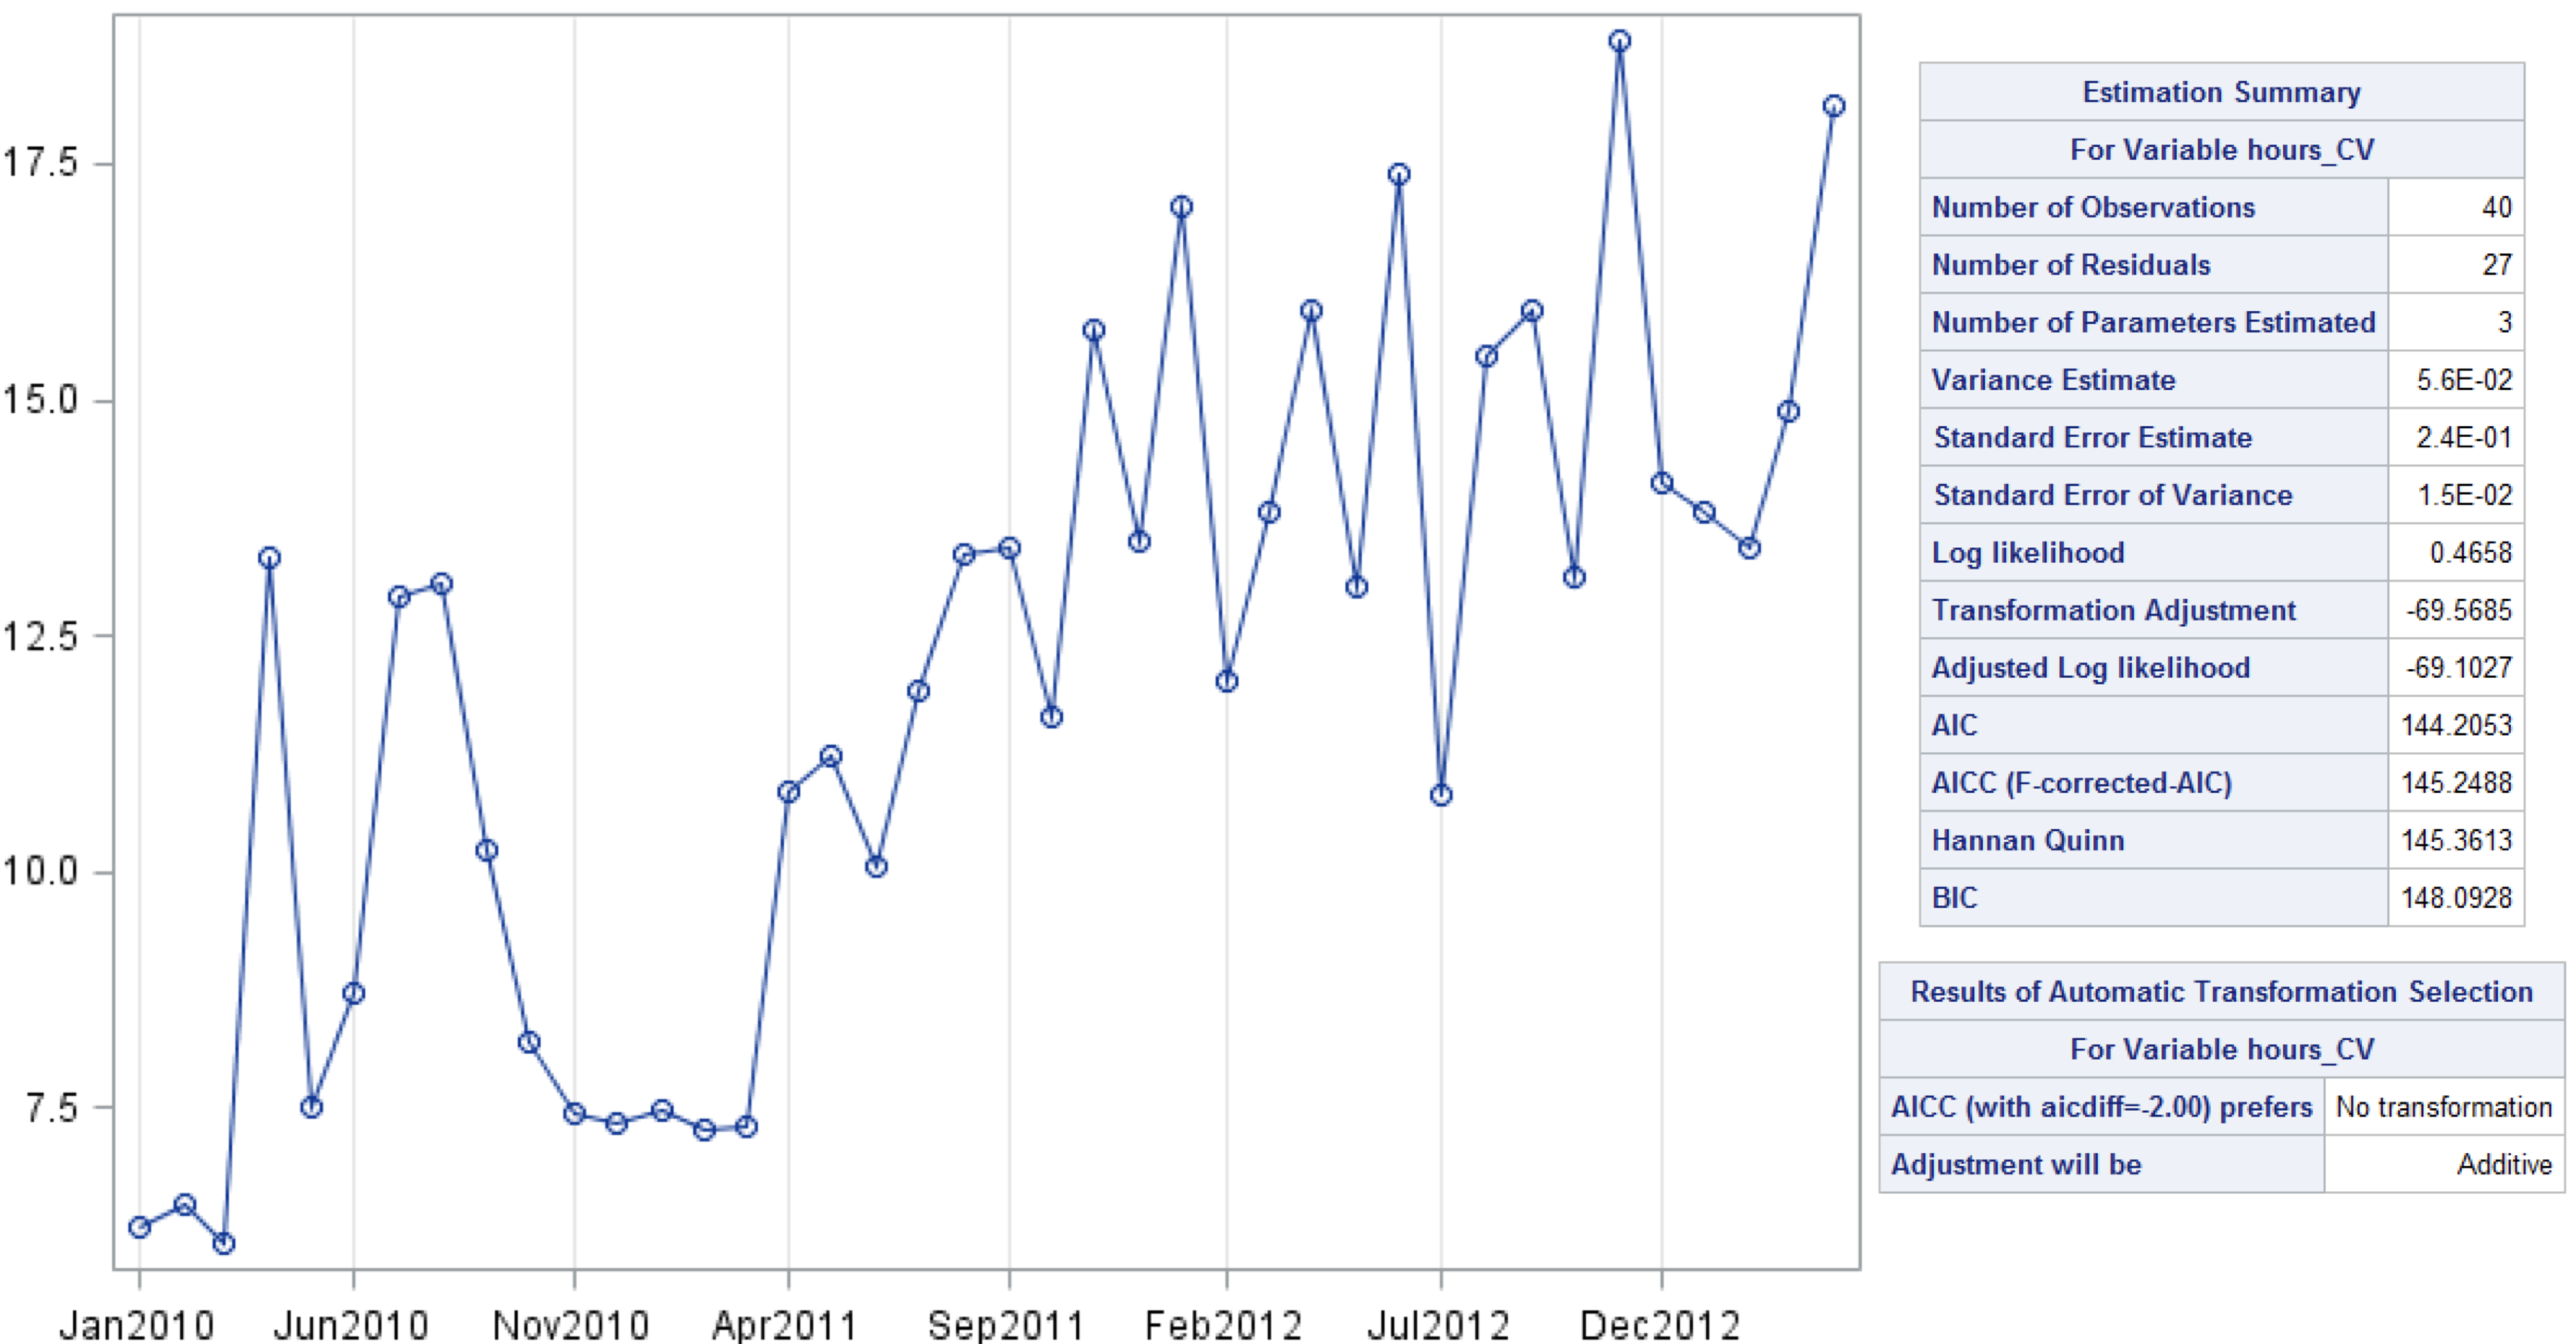
\includegraphics[width=\textwidth]{Images/CV_continuously.png}
\end{center}\newpage \ \\ \noindent A structural break (trend level shift) is identified at OCT2010. \newl The SI (Seasonal Irregular) chart shows that there are more than one irregular component which exhibits volatility.
\begin{center}
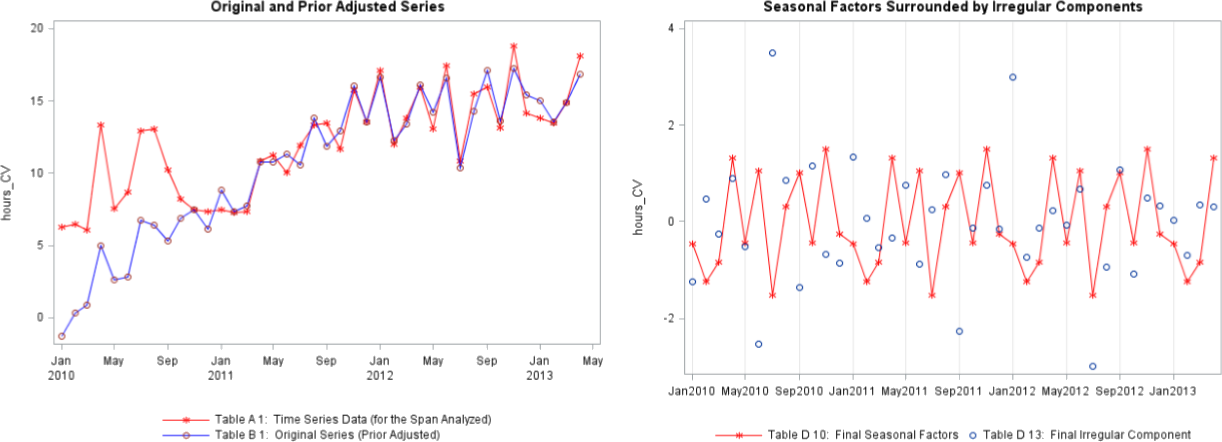
\includegraphics[width=\textwidth]{Images/DiffComponents.png}
\end{center}
\newpage \ \\ \noindent The adjusted series is shown below; the trend and irregular components are also shown separately for readability. \newl It is on the irregular component that detection anomaly would be conducted. 
\begin{center}
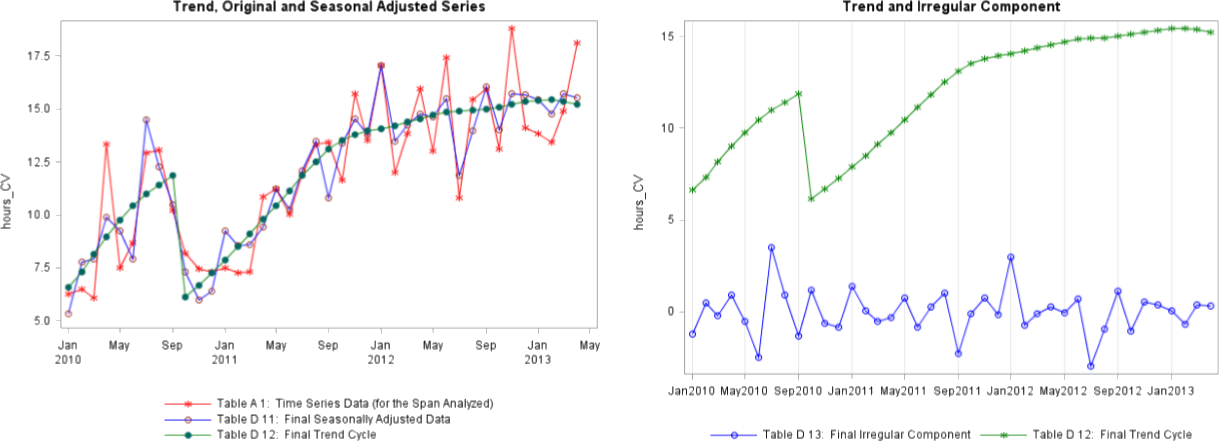
\includegraphics[width=\textwidth]{Images/adjustedplot.png}\end{center} 
\newpage\ \\ \noindent Given that the vast majority of observations in a general problem are typically "normal", another conceptually important approach is to view anomaly detection as a:
\begin{itemize}
\item \textbf{rare occurrence learning} classification problem, or \item  \textbf{novelty detection} data stream problem. \end{itemize} 
While there a number of strategies that use regular classification/clustering algorithms for anomaly detection, they are rarely successful unless they are \textbf{adapted} or \textbf{modified for the anomaly detection context}.
\newl \textbf{MORAL OF THE STORY:} anomaly detection is a difficult problem.
\fh{Basic Concepts}
\noindent Generic systems (think of the monthly transit/dwell times from supply chains) may be realized in 
\begin{itemize}
\item \textbf{normal} states, or  \item \textbf{abnormal} states. 
\end{itemize} 
Normality is not confined to finding the most likely state -- infrequently occurring states could still be normal or plausible under some interpretation of the system. \newpage\ \\ \noindent A system's states are the results of processes or behaviours that follow certain \textbf{natural rules} and \textbf{broad principles}; the observations are a manifestation of these states. \newl Data allows for inferences to be made about the underlying processes, which can be tested or invalidated by the collection of additional data. 
\newl When the inputs are perturbed, the corresponding outputs are likely to be perturbed as well. \newl If anomalies arise from perturbed processes, the \textbf{anomaly detection problem} could be helped along by being able to identify when the underlying process is abnormal. 
\newpage\ \\ \noindent  \textbf{Supervised} anomaly detection algorithms require a \begin{enumerate}
\item \textbf{training set of historical labeled data} on which to build the prediction model (usually costly to obtain), and 
\item testing set on which to evaluate the model's performance in terms of 
\begin{itemize}
\item \textbf{True Positives} ($\text{TP}$)  -- detected anomalies that actually arise from process abnormalities; 
\item \textbf{True Negatives} ($\text{TN}$)  -- predicted normal observations that indeed arise from normal processes; 
\item \textbf{False Positives} ($\text{FP}$)  -- detected anomalies corresponding to regular processes, and 
\item \textbf{False Negatives} ($\text{FN}$) -- predicted normal observations that are in fact the product of an abnormal process.
\end{itemize}
\end{enumerate}
\newpage\ \\ \noindent This is often summarized in a \textbf{confusion matrix}:
\begin{center}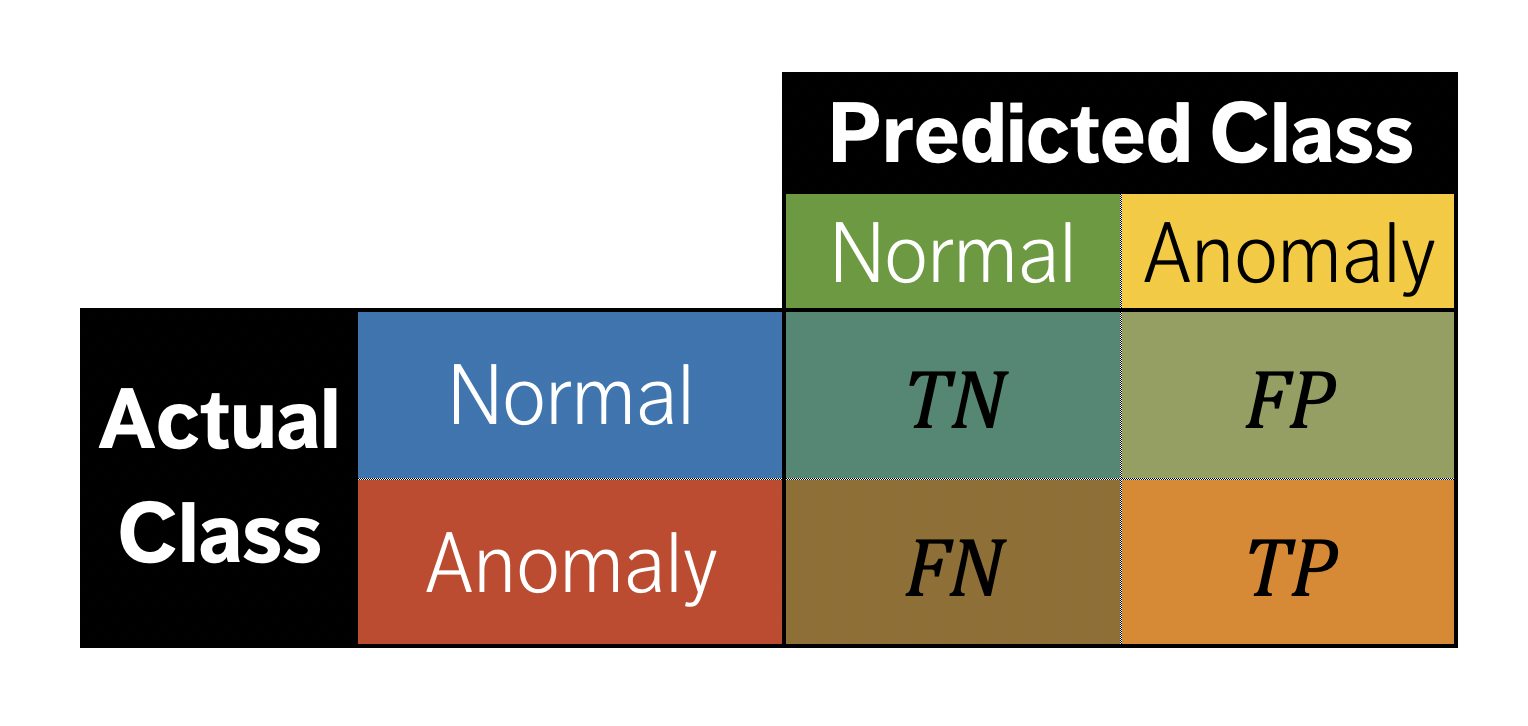
\includegraphics[width=0.6\textwidth]{Images/Confusion_EN.png}\end{center}
Na\"{\i}vely, one might look for an algorithm which maximizes the \textbf{accuracy} $$a=\frac{\text{TN}+\text{TP}}{\text{TN}+\text{TP}+\text{FN}+\text{FP}}.$$ For rare occurrences, this is a losing strategy (see weapon smuggling ex.). \newpage\ \\ \noindent \textbf{Better approach:} try to minimize the FP rate and the FN rate under the assumption that the \textbf{cost of making a false negative error could be substantially higher than the cost of making a false positive error}. \newl 
For a testing set with $d=\text{FN}+\text{TP}$ \textbf{true outliers}, assume that an anomaly detection algorithm identifies $m=\text{FP}+\text{TP}$ \textbf{suspicious observations}, of which $n=\text{TP}$ are \textbf{known} to be true outliers. \newl How well did the algorithm \textbf{perform}?   
\begin{description}
\item[Precision:] proportion of true outliers among suspicious observations $$p=\frac{n}{m}=\frac{\text{TP}}{\text{FP}+\text{TP}};$$ if most of the suspicious points are true outliers, $p\approx 1$;
\newpage\ \item[Recall:] proportion of true outliers detected by the algorithm
$$r=\frac{n}{d}=\frac{\text{TP}}{\text{FN}+\text{TP}};$$ if most of the true outliers are identified by the algorithm, $r\approx 1$;
\item[$F_1-$Score:] harmonic mean of the algorithm's precision and its recall on the testing set 
$$F_1=\frac{2pr}{p+r}=\frac{2\text{TP}}{2\text{TP}+\text{FP}+\text{FN}}.$$
\end{description}
\textbf{Question:} precision, recall, and $F_1-$score do not incorporate $\text{TN}$ in the evaluation process. Is this likely to be a problem? 
\newpage\ \\ \noindent \textbf{Example:} consider a test dataset with $5000$ observations, $100$ of which are anomalous.\newl An algorithm that predicts all observations to be anomalous yields 
\begin{center}
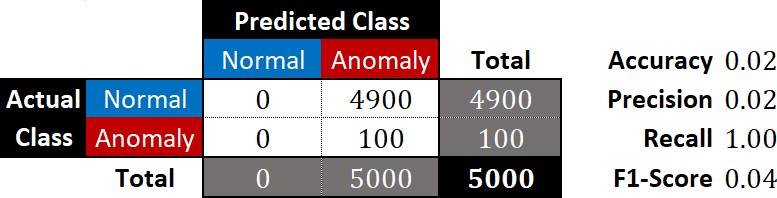
\includegraphics[width=\textwidth]{Images/Ex1.png}
\end{center}
\newpage\ \\ \noindent An algorithm that only detects $10$ of the true outliers and $x$ of the normal observations yields
\begin{center}
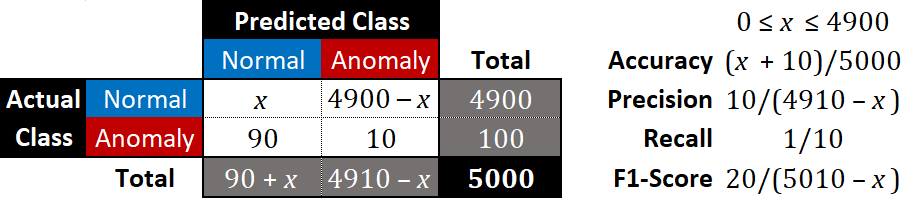
\includegraphics[width=\textwidth]{Images/Ex2.png}\\ \ \\ 
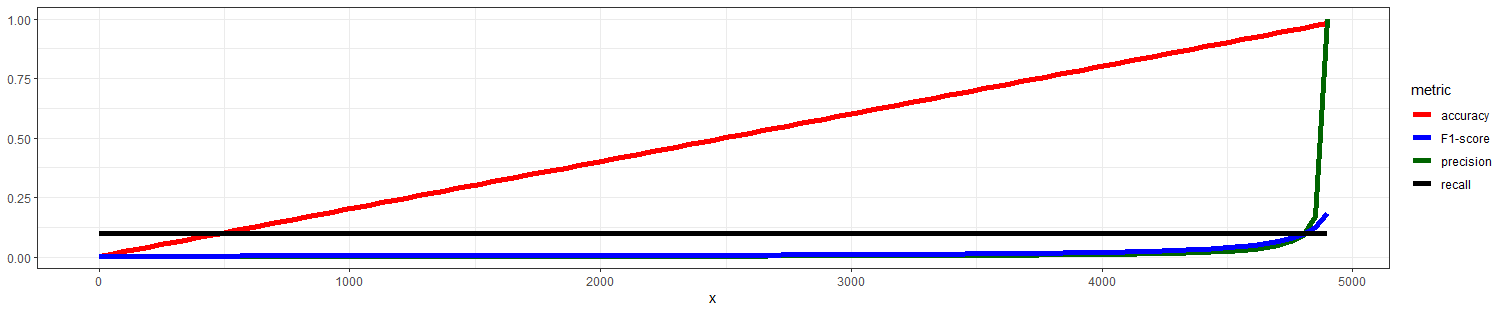
\includegraphics[width=\textwidth]{Images/AODA_metrics.png}
\end{center}
\newpage \ \\ \noindent Another SL approach: estimate the \textbf{relative abnormality} of observations. 
\newl 
Estimating the probability that an observation $\mathbf{x}_1$ is anomalous $\Longrightarrow$ difficult; \\ 
Determining it is more likely to be anomalous than another $\mathbf{x}_2$ $\Longrightarrow$ easier. (We write $\mathbf{x}_1\succeq \mathbf{x}_2$.) \newl Let $k_i\in\{1,\ldots,m\}$ be the rank of the $i^{\text{th}}$ \textbf{true outlier}, $i\in \{1,\ldots,n\}$, in the sorted list of suspicious observations $$\mathbf{x}_1\succeq \mathbf{x}_{k_1}\succeq \cdots\succeq\mathbf{x}_{k_i}\succeq \cdots \mathbf{x}_{k_n}\succeq \mathbf{x}_m,\quad n\leq m;$$ the \textbf{rank power} of the algorithm is $$\text{RP}=\frac{n(n+1)}{2\sum_{i=1}^nk_i}.$$ \newpage\ \\ \noindent When the $n$ actual anomalies are ranked in (or near) the top $n$ suspicious observations, we have $$\sum_{i=1}^nk_i\approx \sum_{i=1}^ni =\frac{n(n+1)}{2} \Longrightarrow \text{RP}\approx 1.$$ As with most performance evaluation metrics, a single raw number is meaningless -- it needs to be compared to other algorithms. \newl Other SL performance evaluation metrics include: 
\begin{itemize}
\item \textbf{AUC} --  the probability of ranking a randomly chosen anomaly higher than a randomly chosen normal observation (higher is better);
\item \textbf{probabilistic AUC} -- a calibrated version of AUC. 
\end{itemize}\newpage \ \\ \noindent On the \textbf{unsupervised} front,  anomalous/normal labels are not used:
\begin{itemize}
\item anomalies are those observations that are dissimilar to other observations;
\item \textbf{clusters} are groupings of similar observations, so 
\item observations without a natural cluster fit are potential anomalies. 
\end{itemize}
\textbf{Challenges:} 
\begin{itemize}
\item most clustering algorithms do not recognize potential outliers (DBSCAN and variants are exceptions), and 
\item finding an appropriate measure of similarity/dissimilarity of observations is difficult (different measures often lead to different cluster assignments).  \end{itemize}
\newpage\  
\begin{center}
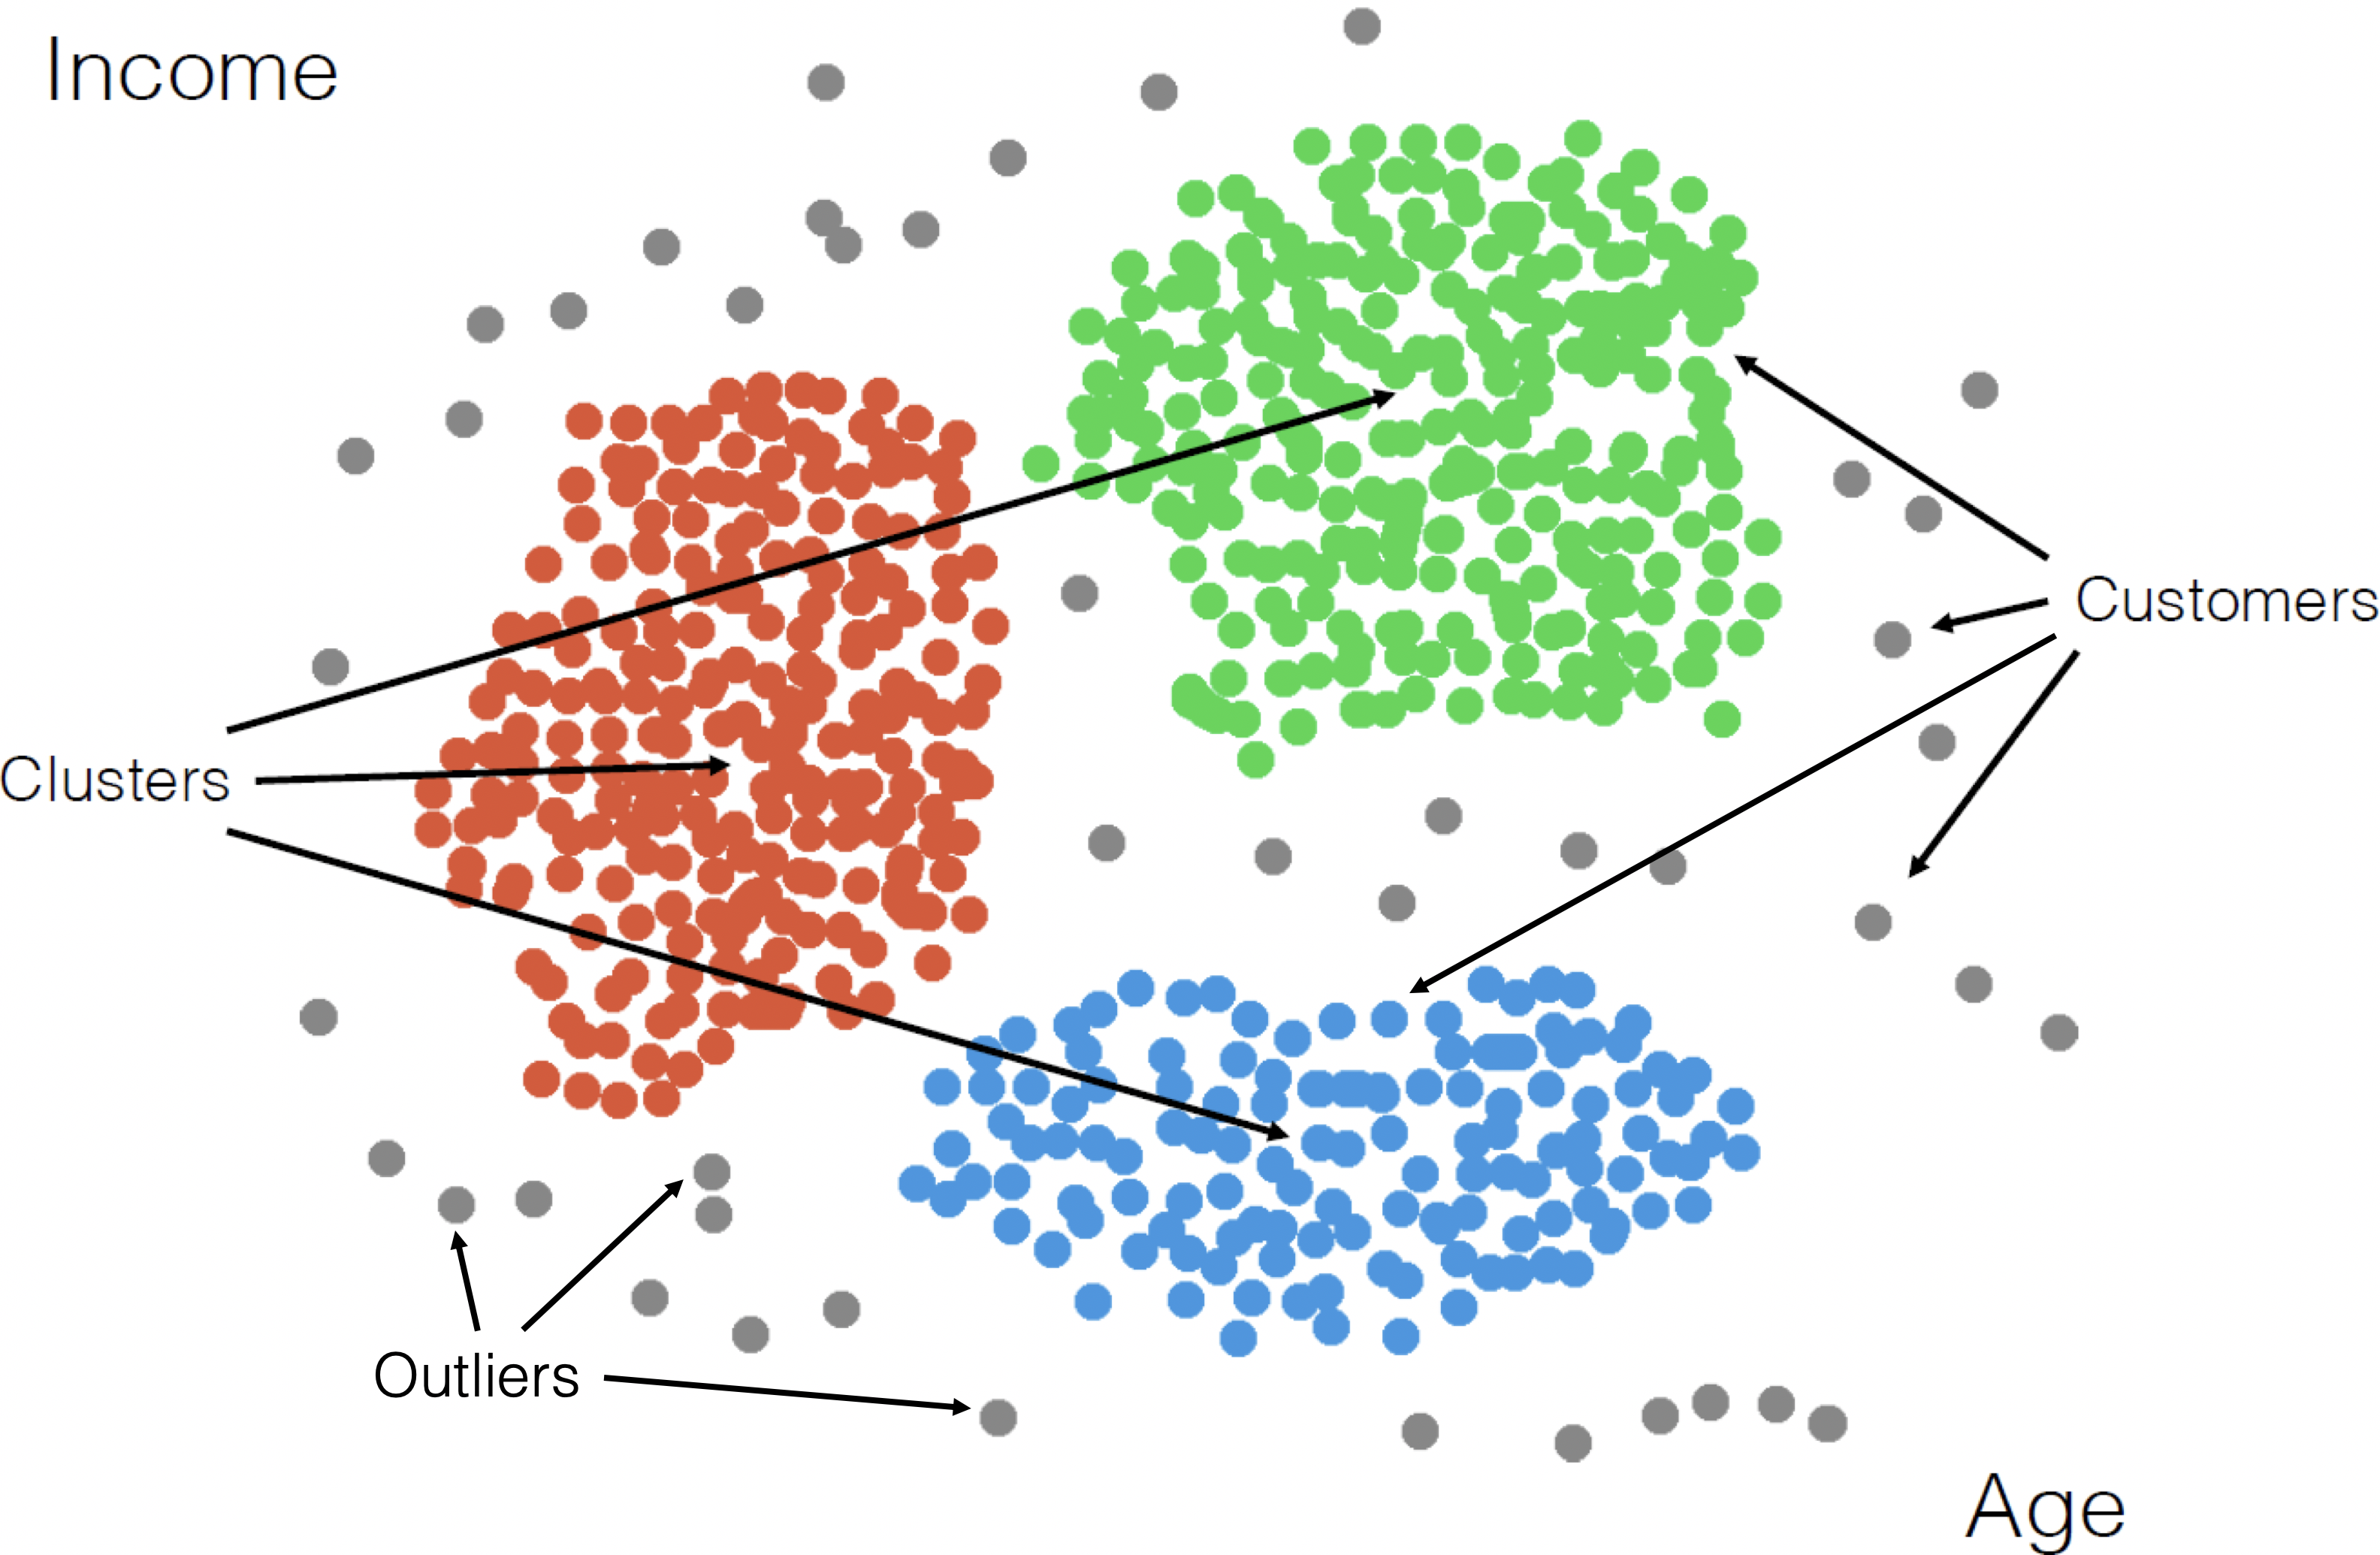
\includegraphics[width=0.75\textwidth]{Images/clustering2_EN.png} \\ 
Clusters of regular customers (red, green, blue) and potential anomalies/outliers (grey) in an artificial dataset.
\end{center}



\fh{\textcolor{darkestgreen}{6.2 -- Quantitative Methods of Anomaly Detection}} \label{6.2} 

\noindent Cluster-based methods are not the only types of UL anomaly detection methods.
\begin{itemize}
\item \textbf{Distance-based methods:} distance to all points, distance to $k$ nearest neighbours ($k$NN),  average distance to $k$NN, median distance to $k$NN, etc.
\item \textbf{Density-based methods:} local outlier factor (LOF), isolation forest, HDBSCAN, etc.
\end{itemize}

\fh{6.2.1 -- Distance-Based Methods} \label{6.2.1}
\noindent We find anomalous observations by  comparing them to other observations (\textbf{anomalies are relative, not absolute}). \newl In the \textbf{distance-based context}, the natural way to compare observations is  to consider their \textbf{distance from a subset of observations}: increasing distance being increasingly \textbf{suggestive} of anomalous status.
\newl \textbf{Requirement:} a \textbf{distance function} or a \textbf{pre-computed table of pair-wise distances} (in discrete case). 
\newl The choice of subsets and distance functions  distinguish the different distance-based algorithms.
\fh{Notation} \begin{itemize}
\item $D \subset \mathbb{R}^n$ is an $n$-dimensional (numerical) data set
\item $\mathbf{p},\mathbf{q}\in D$ are specific observations in $D$
\item $P \subset D$ is a subset of $D$
\item $d: D \times D \to \mathbb{R}$ is a distance function on $D\subset \mathbb{R}^n$
\item the distance between $\mathbf{p}$ and $\mathbf{q}$ is written $d(\mathbf{p},\mathbf{q})$
\item the output of an anomaly detection algorithm is a function $a : D \to \mathbb{R}$
\newpage\ \item $a(\mathbf{p})$ is a number that describes how anomalous $\mathbf{p}$ is \item 
if $a(\mathbf{p}) < a(\mathbf{q})$ for $\mathbf{p},\mathbf{q} \in D$, then $\mathbf{p}$ is \textbf{less anomalous} than $\mathbf{q}$
\item $\alpha \in \mathbb{R}$ is the \textbf{absolute anomaly threshold}
\item  any $\mathbf{p} \in D$ for which $a(\mathbf{p}) > \alpha$ is \textbf{absolutely anomalous}
\end{itemize}
\fh{Similarity Measures}
\noindent A \textbf{similarity measure} is a real-valued function that describes the \textbf{similarity between two objects}.
\newl A common construction for the similarity $w$ between two points $\mathbf{p},\mathbf{q}$: $$w(\mathbf{p},\mathbf{q})=\frac{1}{1+d(\mathbf{p},\mathbf{q})}, \quad \text{for some distance }d.$$ \textbf{Note:}  $w\to 1$ as $d\to 0$, and $w\to 0$ as $d\to \infty$. \newl  
Similarity measures can also be constructed between \textbf{probability distributions} (see Hellinger distance). \newpage\  \begin{center}
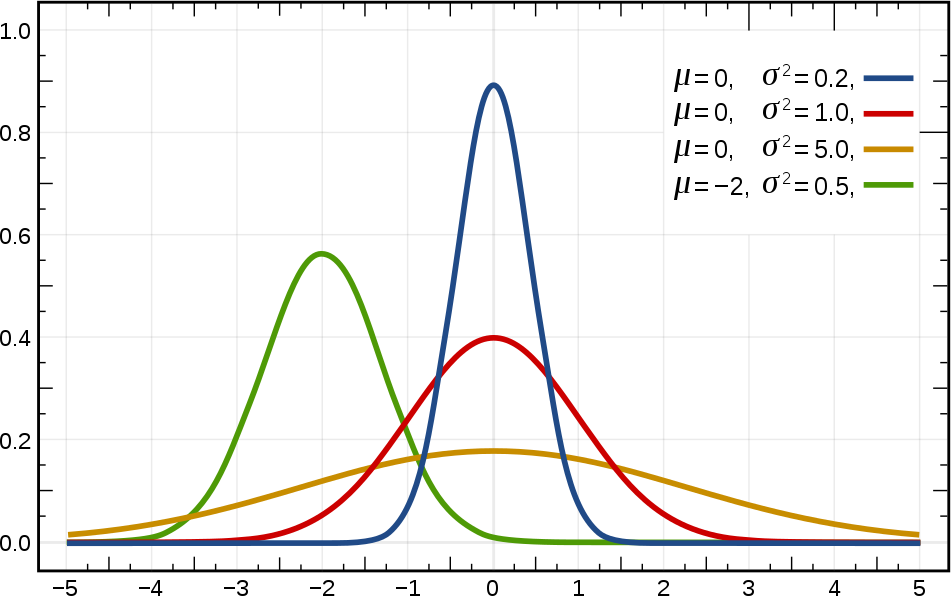
\includegraphics[width=0.8\textwidth]{Images/distributions.png}
\end{center}\newpage \ \\ \noindent
We can think of a single point $\mathbf{p}$ as a probability distribution (with $0\%$ chance of drawing another point). \newl The distance between that point and any other distribution with mean $\mathbf{\mu}$ and covariance matrix $\mathbf{\Sigma}$ can be given using the \textbf{Mahalanobis framework}:

$$
M(\mathbf{p})=\sqrt{(\mathbf{p} - \mathbf{\mu})^{\!\top} \mathbf{\Sigma}^{-1} (\mathbf{p} - \mathbf{\mu}).}
$$

\noindent Alternatively, if $\mathbf{p}$ and $\mathbf{q}$ are drawn from the same distribution with covariance $\Sigma$, then the Mahalanobis distance is a dissimilarity measure between $\mathbf{p}$ and $\mathbf{q}$: 

$$
d_M(\mathbf{p},\mathbf{q})=\sqrt{(\mathbf{p} - \mathbf{q})^{\!\top} \mathbf{\Sigma}^{-1} (\mathbf{p} - \mathbf{q}).}
$$
\newpage\ \\ \noindent 
\textbf{Example:} consider a 4D-dataset drawn from a multivariate  $\mathcal{N}(\mathbf{\mu},\mathbf{\Sigma})$ with  
\small $$\mathbf{\mu}=(1,-2,0,1),\quad \mathbf{\Sigma}=\begin{pmatrix}1 & 0.5 & 0.7 & 0.5 \\ 0.5 & 1 & 0.95 & 0.3 \\ 0.7 & 0.95 & 1 & 0.3 \\ 0.5 & 0.3 & 0.3 & 1\end{pmatrix}.$$\normalsize
$100$ observations $\mathbf{p}_1$ to $\mathbf{p}_{100}$ are ``normal'': 
\small \begin{center}
\begin{tabular}{crrrr}
\textbf{stat} & $x_1\ \ $ & $x_2\ \ $ & $x_3\ \ $ & $x_4\ \ $ \\ \hline          
 min   & $-1.9049$  & $-4.4113$ & $-2.5324$ & $-1.9949$ \\ 
 $Q_1$ &  $ 0.3812$  & $-2.6464$ & $-0.6190$ & $ 0.3361$ \\ 
 med   &  $ 0.9273$  & $-2.0220$ & $-0.0506$ & $ 0.9381$ \\ 
 avg  &  $ 0.9374$  & $-1.9788$ & $ 0.0071$ & $ 0.9438$ \\ 
 $Q_3$ &  $ 1.4615$  & $-1.4002$ & $ 0.6296$ & $ 1.5906$ \\ 
 max   &  $ 3.4414$  & $0.5223$  & $ 2.0265$ & $ 2.8073$ \\
 \end{tabular}
\end{center}\normalsize
$2$ observations are ``anomalous'':  $\mathbf{z}_1=(1,1,1,1)$, $\mathbf{z}_4=(4,4,4,4)$. 
\newpage\ \begin{center}
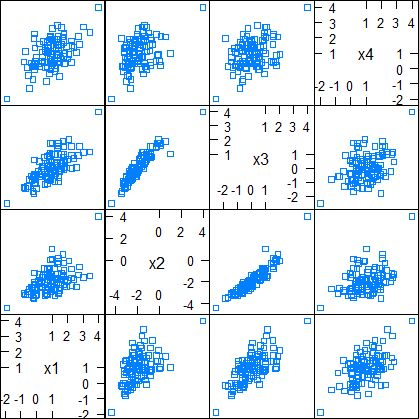
\includegraphics[height=0.8\textheight]{Images/Artificial_4D_Dataset} \\ Visually, it seems there might be $3$ outliers. 
\end{center} \newpage\ \begin{center}
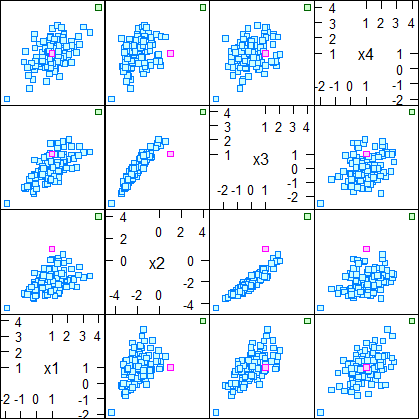
\includegraphics[height=0.92\textheight]{Images/Artificial_4D_Dataset_Groups}
\end{center}\newpage\ \\ \noindent In general, the mean vector and the covariance structure must be estimated from the data: 
\small $$\mathbf{\hat{\mu}}=(0.968, -1.891,0.056,0.974),\quad \mathbf{\hat{\Sigma}}=\begin{pmatrix}
0.900 & 0.569 & 0.665 &  0.503 \\
0.569 & 1.312 & 1.069 &  0.469 \\
0.665 & 1.069 & 0.992 &  0.397 \\
0.503 & 0.469 & 0.397 &  0.904 \end{pmatrix}.$$\normalsize
These are distinct from $\mathbf{\mu}$ and $\mathbf{\Sigma}$, but close enough to be explained by 
\begin{itemize}
\item sampling variation
\item $\mathbf{z}_1,\mathbf{z}_4\not\sim \mathcal{N}(\mathbf{\mu},\mathbf{\Sigma})$
\end{itemize}
To identify anomalous observations, compute the Mahalanobis distance from all points to the empirical distribution, and between all pairs.  
\newpage\ \begin{center}
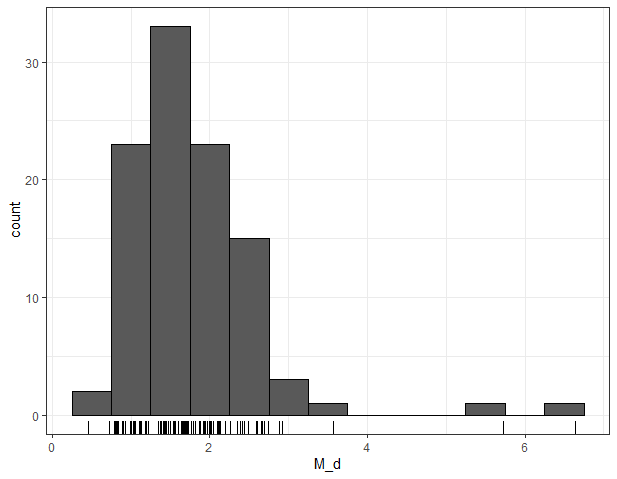
\includegraphics[height=0.8\textheight]{Images/Histogram_Md} \\ Histogram of Mahalanobis distances to empirical distribution.
\end{center}
\newpage\ \begin{center}
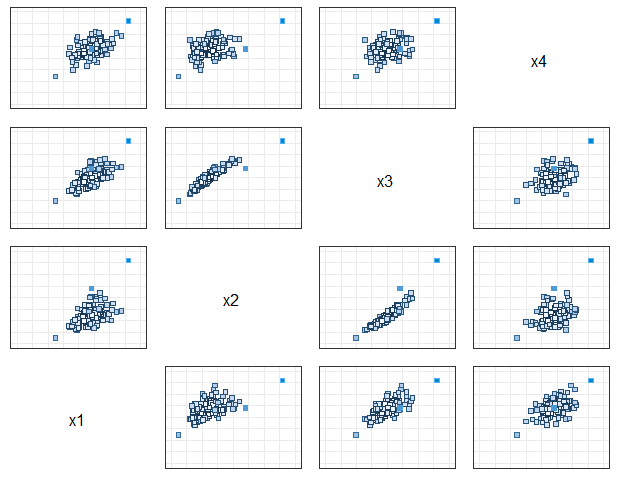
\includegraphics[height=0.85\textheight]{Images/Artificial_4D_Dataset_Md_scores} \\ Scatter plot of Mahalanobis distances to empirical distribution.
\end{center}\newpage\ \\  \begin{center}
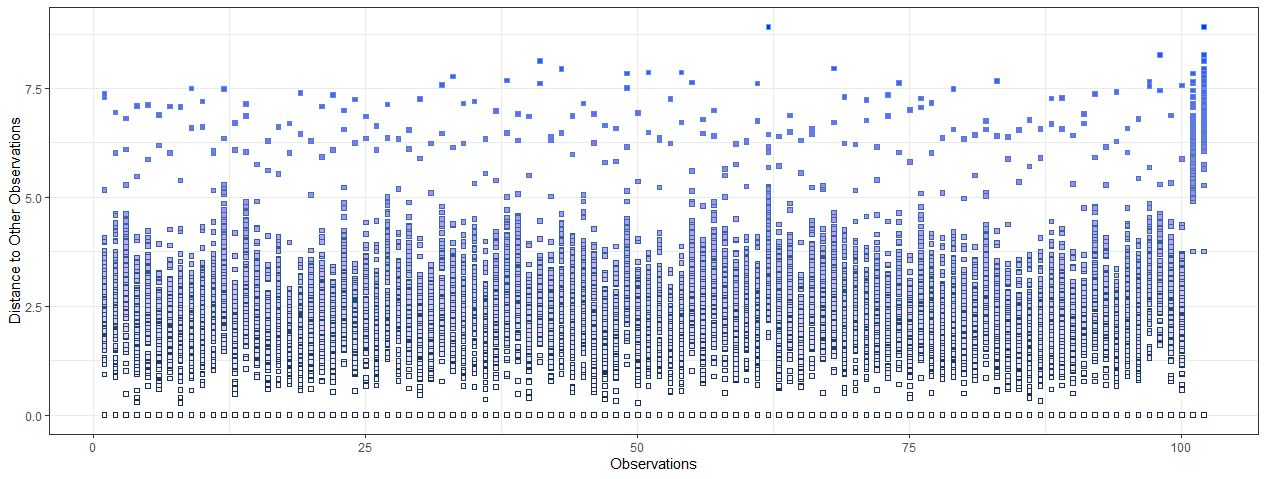
\includegraphics[width=\textwidth]{Images/Artificial_4D_Datasets_Pairs} \\ Mahalanobis distances between each pair (empirical distribution). \\ Notice observations $101$ and $102$, as well as the diffuse cloud of points above the value $5.0$.
\end{center}\newpage\ \\  \begin{center}
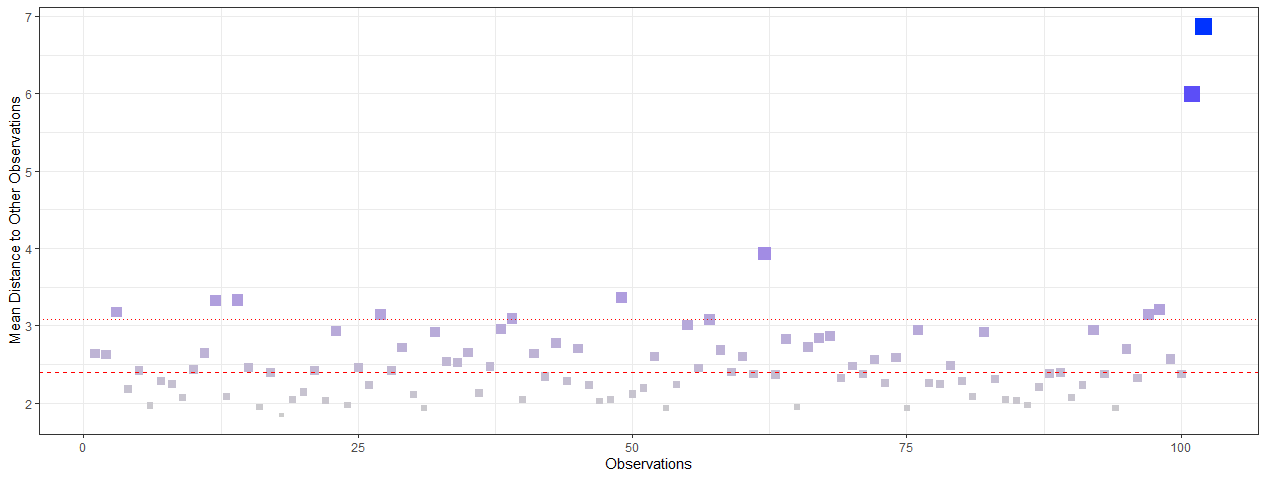
\includegraphics[width=\textwidth]{Images/Artificial_4D_Dataset_MeanDist} \\ Mean Mahalanobis distances between each pair (empirical distribution). \\ Notice observations $101$ and $102$ again. The red lines represent the median mean distance, and $1$ standard deviation the median mean distance. \\ The Mahalanobis framework seems to identify $2$ outliers. 
\end{center}\newpage\ \\ \noindent If  $\Sigma$ is diagonal, then 

$$
d_M(\mathbf{p},\mathbf{q})=\sqrt{\sum_{i=1}^n \frac{(p_i - q_i)^2}{\sigma_i^2}},
$$
where $\sigma_i^2$ is the variance along the $i$-th dimension.
\newl If $\Sigma$ is the identity matrix, then we recover the \textbf{Euclidean distance}

$$
d_2(\mathbf{p},\mathbf{q})=\sqrt{\sum_{i=1}^n (p_i - q_i)^2}.
$$
\noindent In an anomaly detection context, a \textbf{linear normalization} is usually applied to each dimension so that each entry lies in the hypercube  $[-1,1]^n$.
\newpage\ \\ \noindent The \textbf{Minkowski distance} of order $p$ is a generalization of the Euclidean distance:
$$
d_p(\mathbf{p},\mathbf{q})=\left( \sum_{i=1}^n |p_i - q_i|^p \right)^{1/p}.
$$
\begin{itemize}
\item For $p=1$, we recover the \textbf{Manhattan distance}: $$d_1(\mathbf{p},\mathbf{q})=\sum_{i=1}^n|p_i-q_i|;$$ 
\item for $p=\infty$, we recover the \textbf{supremum} (Chebychev) \textbf{distance} $$d_{\infty}(\mathbf{p},\mathbf{q})=\max_{i=1}^n \left\{|p_i - q_i|\right\}.$$ 
\end{itemize}
\newpage\ \\ \noindent The Minkowski distance $d_p$ is only an actual distance function (a \textbf{metric}) when  $p \geq 1$, but an exception is made for 
$$
d_{-\infty}(\mathbf{p},\mathbf{q})=\min_{i=1}^n \left\{|p_i - q_i|\right\}.
$$
When working with categorical data (such as in one-hot encoding of text), it can be useful to use distances for binary vectors.\newl  Let $\mathbf{p},\mathbf{q}\in  \{0,1\}^n$.\newl 
The \textbf{Hamming distance} between $\mathbf{p}$ and $\mathbf{q}$ counts the number of positions where they differ: 
$$d_H(\mathbf{p},\mathbf{q})=\sum_{i=1}^n|p_i-q_i|.$$
\newpage\ \\ \noindent The \textbf{Jaccard similarity} of two datasets $P$ and $Q$, is defined as the size of their intersection divided by the size of their union
$$
J(P,Q)
= \frac{|P \cap Q|}{|P \cup Q|}
= \frac{|P \cap Q|}{|P| + |Q| - |P \cap Q|}
$$
Their \textbf{Jaccard distance} is $d_J(P,Q)=1 - J(P,Q)$. This can be extended to binary vectors $\mathbf{p}$ and $\mathbf{q}$. \newl Consider an arbitrary set $D=\{x_1,x_2,\ldots,x_n\}$. We build $P$ as follows: if $p_i=1$ then $x_i\in P$; otherwise $x_i\not\in P$. Similarly for $Q$. \newl Then $|P|=\sum p_i$, $|Q|=\sum q_i$, $|P\cap Q|=\sum p_iq_i=\mathbf{p}\cdot\mathbf{q}$ and  
$$d_J(\mathbf{p},\mathbf{q})=d_J(P,Q)=1-J(P,Q)=1-\frac{\mathbf{p}\cdot \mathbf{q}}{\sum (p_i+q_i)-\mathbf{p}\cdot \mathbf{q}}.$$ 
\newline\newline
Finally, let $\mathbf{p},\mathbf{q}\neq \mathbf{0}$. Recall that 
$\mathbf{p} \cdot \mathbf{q} 
= \lVert p \rVert \lVert q \rVert \cos\theta,$
where $\theta$ is the angle between $\mathbf{p}$ and $\mathbf{q}$.\newl  The \textbf{cosine similarity} between $\mathbf{p}$ and $\mathbf{q}$ is 
$$
\cos\theta
= \frac{p \cdot q}{\lVert p \rVert \lVert q \rVert}
= \frac{\sum_{i=1}^n p_i q_i}{\sqrt{\sum_{i=1}^n p_i^2} \sqrt{\sum_{i=1}^n q_i^2}}.
$$
This also holds $\mathbf{p},\mathbf{q}$ are non-binary. The value ranges between $1$ and $-1$:
\begin{itemize}
\item $\cos \theta= 1$ when $\mathbf{p}=\mathbf{q}$;
\item $\cos \theta= -1$ when $\mathbf{p}=-\mathbf{q}$, and \item $\cos \theta =0$ when $\mathbf{p}$ and $\mathbf{q}$ are perpendicular.
\end{itemize}
\newpage
\begin{center}
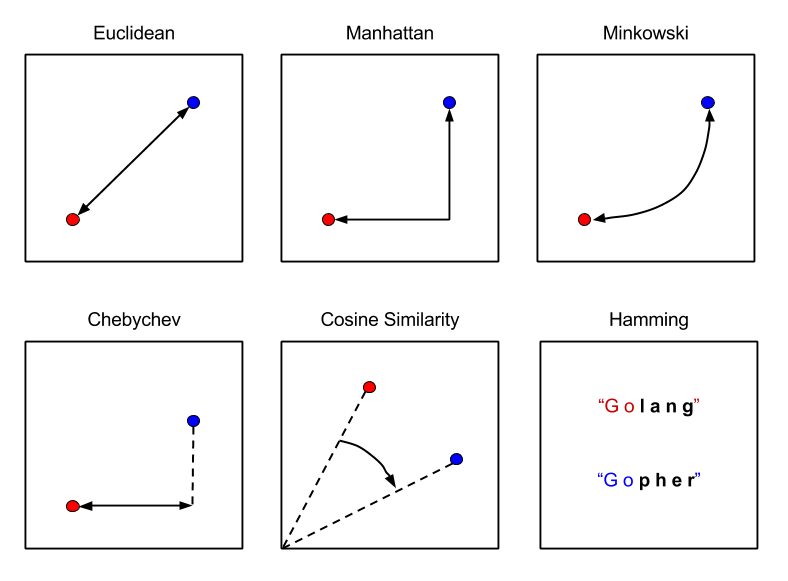
\includegraphics[width=0.9\textwidth]{Images/distances_comparison}
%Machine Learning with Go, Whitenack
\end{center}
\fh{Distance-Based Approaches}
\normalsize \noindent Finding the right distance function to use for anomaly detection is \textbf{NOT AN EASY TASK} -- contextual understanding and domain expertise are required.\newl  
Any such distance function can be used as the basis for anomaly detection algorithms (the ideas can also be extended to more complex algorithms).
\newline\newline Given some distance function $d$, dataset $D$, and integers $k,\nu\leq |D|$, 
the \textbf{distance to all points} anomaly detection algorithm considers each point $\mathbf{p}$ in $D$ and adds the distance from $\mathbf{p}$ to every other point in $D$, i.e.
$$
a(\mathbf{p}) 
= \sum_{\mathbf{q}\neq \mathbf{p} \in D} d(\mathbf{q}, \mathbf{p}).
$$
\newpage\ \\ \noindent The $\nu$ points with largest values for $a$ are then said to be \textbf{anomalous according to} $a$. \newl This approach often selects the most extreme observations as anomalous, which may be of limited use in practice. 
\newl The \textbf{distance to nearest neighbour} algorithm uses 
$$
a(\mathbf{p}) 
= \min_{\mathbf{q}\neq \mathbf{p} \in D} \{d(\mathbf{q}, \mathbf{p})\},
$$
with a similar definition for the $\nu$ anomalous points. 
\newl The \textbf{average distance to $k$ nearest neighbours} and \textbf{median distance to $k$ nearest neighbours} are defined similarly. 




\fh{6.2.2 -- Density-Based Methods} \label{6.2.2} 


Density-based approaches, on the other hand, view points as anomalous if they occur in \textbf{low density regions}.
% Three density-based methods are presented in this section, however there are many 

\fh{Local Outlier Factor} % p110
\begin{center}
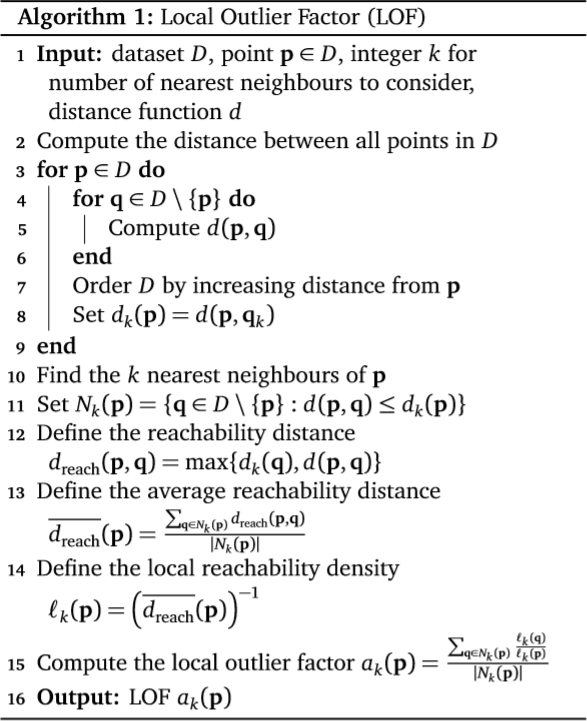
\includegraphics[height=\textheight]{Images/Algorithm1}
\end{center}
The \textbf{Local Outlier Factor} (LOF) algorithm was proposed in 2000 by \cite{LOF} 
(a summary can be found in Section 6.4.2 of \cite{A10}). 
LOF works by measuring the local deviation of each point in a dataset from its $k$ nearest neighbours, with a point said to be anomalous if this \textbf{deviation is large}.

A \textbf{local $k-$region} around a point $\mathbf{p}$ is defined as the $k$ nearest neighbours of $\mathbf{p}$. The density of points in each of their respective local $k-$neighbourhoods is estimated, and compared to the density of the local $k-$neighbourhoods of the point within their own $k-$neighbourhood.

This can then be used to identify outliers that inhabit regions of lower density than their neighbours,
as $\mathbf{p}$ would be in Figure \ref{lofoutlier}. The formal procedure is shown in Algorithm~\ref{alg:LOF}. 

\begin{center}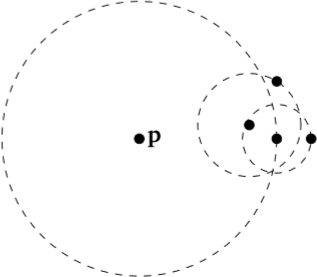
\includegraphics[width=0.5\textwidth]{Images/Figure11}
\end{center}
{For $k=2$, $\mathbf{p}$ is an outlier as it has lower density than its neighbours.}

\noindent LOF is able to identify \textbf{local outliers}, but selecting a threshold beyond which a point is considered an outlier is difficult. \newl LOF introduces the idea of a \textbf{reachability distance}, which improves the stability of results within clusters/regions: within a local $k-$region around $\mathbf{p}$, it is simply the maximal distance to its $k-$neighbours; outside of that region, it is the actual distance from $\mathbf{p}$. 
\par In Figure \ref{reachability} (with $k=3$), for instance, the points $\mathbf{q}_1, \mathbf{q}_2, \mathbf{q}_3$ all have the same reachability distance from $\mathbf{p}$ as they are all $3$-neighbours of $\mathbf{p}$, that is, 
$$
d_{\text{reach}}(\mathbf{p}, \mathbf{q}_1) 
= d_{\text{reach}}(\mathbf{p}, \mathbf{q}_2)
= d_{\text{reach}}(\mathbf{p}, \mathbf{q}_3)
= d(\mathbf{p}, \mathbf{q}_3)
.$$
The point $\mathbf{q}_4$, on the other hand, has 
$d_{\text{reach}}(\mathbf{p}, \mathbf{q}_4)
= d(\mathbf{p}, \mathbf{q}_4)
$
as it is not a $k$-neighbour of $\mathbf{p}$.

\begin{center}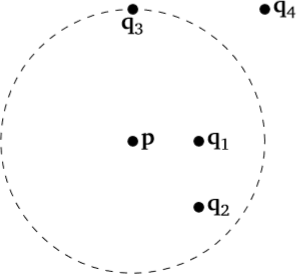
\includegraphics[width=0.5\textwidth]{Images/Figure12}
\end{center}
{The region of uniform reachability distance around $\mathbf{p}$ for $k=3$.}

\fh{DBSCAN}
Density-Based Spatial Clustering of Applications with Noise (DBSCAN) was proposed in 1996 by \cite{DBSCAN} 
(a summary can be found in Section 4.1.5 of \cite{A10}). 
As its name suggests, it is a density-based clustering algorithm that groups nearby points together and labels points that do not fall in the clusters as \textbf{anomalies}.

Hierarchical DBSCAN (HDBSCAN) \cite{HDBSCAN} was introduced in 2013.
It notably removes the problem of choosing the parameter for the radius of a neighbourhood by considering all possible radii. 
Further documentation can be found at \cite{HDBSCAN_code}. \newl 
In DBSCAN, 
\begin{itemize} 
\item a point $\mathbf{p}$ is a \textbf{core point} if there are a minimum number $m$ of points within distance $r$ of $\mathbf{p}$;
\item a point $\mathbf{q}$ is a \textbf{border point} if it is not itself a core point but is within distance $r$ of one, and 
\item a point $\mathbf{o}$ is an \textbf{outlier} if it is neither a core nor a border point.
\end{itemize}

\begin{center}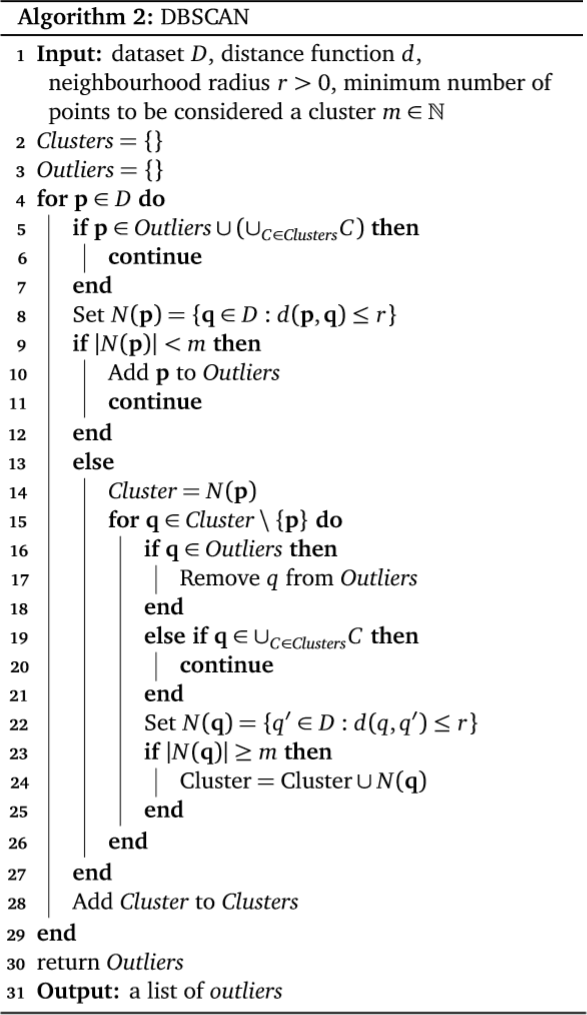
\includegraphics[height=\textheight]{Images/Algorithm2}
\end{center}







\begin{center}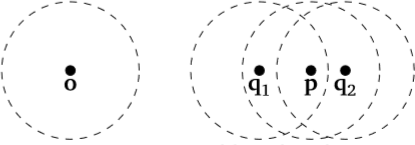
\includegraphics[width=0.5\textwidth]{Images/Figure13}
\end{center}
{For minimum neighbourhood size $m=2$ and this fixed radius $r$, $\mathbf{o}$ is an outlier, $\mathbf{p}$ a core point, and $\mathbf{q}_1$ and $\mathbf{q}_2$ are border points.}

DBSCAN considers each point in the dataset individually. If that point is an outlier, then it is added to a list of outliers. Otherwise if it is a core point, then its $r$-neighbourhood forms the beginning of a new cluster. Each point in this $r$-neighbourhood is then considered in turn, with the $r$-neighbourhoods of other core points contained in the neighbourhood being added to the cluster. \par This expansion repeats until all points have been examined. During this step points that were previously labelled as outliers may be updated as they become border points in this new cluster. This process continues until every point has either been assigned to a cluster or labelled as an outlier (see Algorithm~\ref{dbscan} and Figure~\ref{DBSCANlabels}).

While DBSCAN's dual use as a clustering algorithm may seem irrelevant in the outlier detection setting,
its ability to succesfully identify clusters is crucial to being able to label the remaining points as outliers.
\newl 
On the one hand, in DBSCAN the number of clusters does not need to be known beforehand (unlike in $k-$means and other clustering algorithms) and clusters of arbitrary shape can be detected. \par Furthermore, when using HDBSCAN, only the parameter for the minimum cluster size $m$ is required, which can be set fairly intuitively, which is not the case for the parameters in general clustering algorithms: if the elements of $D$ are $n-$dimensional, take $m\geq n+1$ (larger values of $m$ allow for better noise identification).
\newl On the other hand, DBSCAN is not deterministic, as border points can be assigned to different clusters depending on the order in which core points are considered (this does not affect its use as an anomaly detection algorithm, however).
\par In high dimensions, the ability of any distance function based on Euclidean distance to distinguish near and distant points diminishes due to the \textbf{Curse of Dimensionality}; thus in high dimension spaces, it  become ineffective (as do  other clustering algorithms). \par  Finally, DBSCAN cannot handle differences in local densities as the radius of a neighbourhood $r$ is fixed; this could lead to sparser clusters being labelled as outliers, or to outliers surrounding a denser cluster being included in the cluster.
This issue is overcome in HDBSCAN.

\fh{Isolation Forest}
The previously discussed approaches first construct models of what normal points look like, and then identify points that do not fit this model.
The Isolation Forest algorithm \cite{A15} introduced in 2008 instead tries to explicitly identify outliers under the assumptions that there are few outliers and that these outliers have very different attributes compared to normal points. Doing so allows the use of sampling techniques that increase algorithmic speed while decreasing memory requirements.
\begin{center}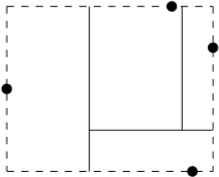
\includegraphics[width=0.5\textwidth]{Images/Figure14}
\end{center}
{A partitioning constructed during Isolation Tree generation.}

The Isolation Forest algorithm tries to isolate anomalous points. It does this by randomly selecting an attribute and then randomly selecting a split value between that attribute's min and max values. This recursively partitions the points until every point is isolated in its own partition.
\newl Recursive partitioning yields a binary tree called an \textbf{Isolation Tree}. The root of this tree is the entire dataset; each node is a subset of the observations, and each branch corresponds to one of the generated partitions. The leaf nodes are singleton sets containing a single isolated point. Each point is then assigned a score derived from how deep in the tree its singleton partition appears (see Figure~\ref{isolationtree} and Algorithm~\ref{iTree}). 
\par As points that are shallower in the tree were easier to separate from the rest, these are the likely \textbf{outliers}. Since only shallow points are of interest, once the height of the tree has reached a given threshold (the expected height of a random binary tree, say), further construction of the tree can be stopped to decrease computational cost. \par 
Additionally, instead of building a tree from the entire dataset, a tree can be constructed from a subset. The location of any point within this smaller tree can then be estimated, again saving computational and memory resources. These two improvements are detailed in the original paper \cite{A15}. 
\newl Once a number of Isolation Trees have been randomly generated (\textbf{Isolation Forest}), a score can be computed for each point. This is done by searching each tree for the location of a given point and noting the path length required to reach it. Once a point's path length in each tree has been computed, the average path length is taken to be its score.
\newpage\noindent  It can be desirable to construct a normalized anomaly score that is independent of the size of the dataset.

\begin{center}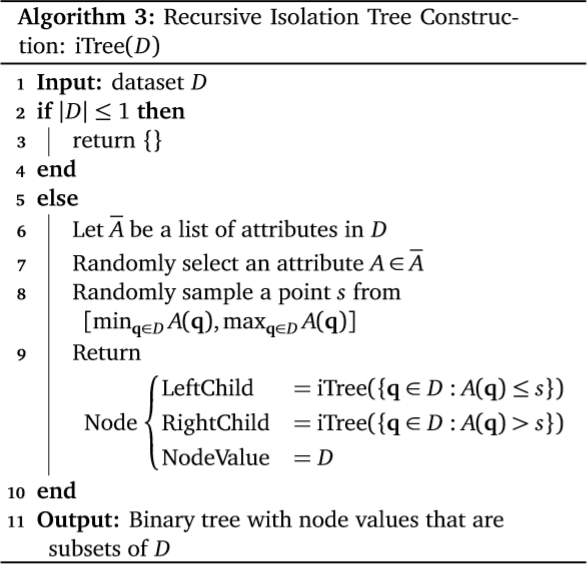
\includegraphics[height=\textheight]{Images/Algorithm3}
\end{center}
\begin{center}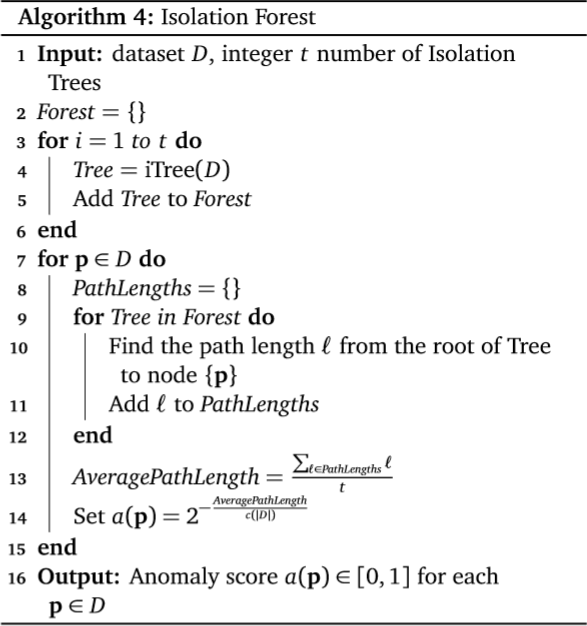
\includegraphics[height=\textheight]{Images/Algorithm4}
\end{center}

In order to do this, the expected path length of a random point in an Isolation Tree (i.e. binary tree) must be estimated. With $n = |D|$, it can be shown that the expected length is 
$$
c(n) 
= 2 H(n-1) - \frac{2(n-1)}{n},
$$
where $H(n-1)$ is the $(n-1)^{\text{th}}$ harmonic number, which can be approximated by $\ln(n-1) + 0.577$;
$c(n)$ is then used to normalize the final anomaly score $a(\mathbf{p})$ for $\mathbf{p} \in D$, which is given by
$$
\log_2 a(\mathbf{p})
= -\frac{\text{average path length to $\mathbf{p}$ in the Isolation Trees}}{c(n)}.
$$
Thus defined, $a(\mathbf{p})\in [0,1]$, with $a(\mathbf{p}) \approx 1$ suggesting $\mathbf{p}$ is an \textbf{anomaly}, $a(\mathbf{p}) \leq 0.5$ suggesting $\mathbf{p}$ is a normal point;
if all points receive a score around $0.5$, this suggests that there are no anomalies present.
\newl Isolation Forests have small time and memory requirements; can handle high dimensional data, and do not need observations to have been labeled anomalies in the training set, but the anomaly score assigned to a given point can have high variance over multiple runs of the algorithm. The authors of \cite{EIF} propose some solutions.
\begin{center}\rule{0.5\linewidth}{.4pt}\end{center}
In general, \text{density-based} schemes are more powerful than distance-based schemes when a dataset contains patterns with diverse characteristics, but less effective when the patterns are of comparable densities with the outliers \cite{JZ}.




\fh{\textcolor{darkestgreen}{
6.3 -- Qualitative Methods}} \label{6.3} 



\fh{6.3.1 -- Definitions and Challenges} \label{6.3.1} 



\fh{6.3.2 -- Review of Methods} \label{6.3.2} 





\fh{\textcolor{darkestgreen}{6.4 -- Anomalies in High-Dimensional Datasets}} \label{6.4}



\fh{6.4.1 -- Definitions and Challenges} \label{6.4.1}



\fh{6.4.2 -- Projection-Based Methods} \label{6.4.2} 



\fh{6.4.3 -- Subspace  Methods} \label{6.4.3}



\fh{\textcolor{darkestgreen}{6.5 -- Applications}} \label{6.5}



\fh{6.5.1 -- S\&P 500} \label{6.5.1}



\fh{6.5.2 -- Airports} \label{6.5.2} 



\fh{6.5.3 -- Application 3} \label{6.5.3} 



\fh{6.5.4 -- Application 4} \label{6.5.4} 



\fh{6.5.5 -- Application 5} \label{6.5.5} 





\fh{\textcolor{darkestgreen}{6.6 -- Advanced Topics}} \label{6.6}



\fh{6.6.1 -- Outlier Ensembles} \label{6.6.1}



\fh{6.6.2 -- Anomalies in Text Datasets Methods} \label{6.6.2} 


\end{document}


